\documentclass[a4paper, 12pt, oneside]{report}

\usepackage{graphicx}
\usepackage{float}
\usepackage[table,xcdraw]{xcolor}
\usepackage[utf8]{inputenc}
\DeclareUnicodeCharacter{20B9}{\text{Rs.\,}}
\usepackage[T1]{fontenc}
\usepackage{fouriernc}
\usepackage{subcaption}
\usepackage{longtable}
\usepackage[nottoc]{tocbibind}
\usepackage{url}
\usepackage{hyperref}
\usepackage{amsmath}
\usepackage{amssymb}
\usepackage{booktabs}
\usepackage{array}
\usepackage{sectsty}
\sectionfont{\raggedright}
\subsectionfont{\raggedright}
\subsubsectionfont{\raggedright}
\paragraphfont{\raggedright}
\usepackage{tikz}
\usetikzlibrary{arrows.meta, positioning, fit, backgrounds, calc}
\tikzset{
  tierbox/.style={
    rectangle,
    rounded corners=5pt,
    draw=black!70,
    line width=0.8pt,
    font=\small,
    inner sep=8pt
  },
  tierframe/.style={
    rectangle,
    rounded corners=6pt,
    draw=black!60,
    line width=0.8pt,
    dashed,
    inner sep=12pt
  },
  arrowflow/.style={
    -{Latex[length=2.5mm, width=1.8mm]},
    draw=black!80,
    line width=0.8pt,
    shorten >= 6mm,
    shorten <= 6mm
  }
}
\usepackage{listings}
\lstdefinelanguage{JavaScript}{
  keywords={break, case, catch, continue, debugger, default, delete, do, else, finally, for, function, if, in, instanceof, new, return, switch, this, throw, try, typeof, var, void, while, with, let, const, async, await},
  morecomment=[l]{//},
  morecomment=[s]{/*}{*/},
  morestring=[b]',
  morestring=[b]",
  sensitive=true
}
\lstset{
  basicstyle=\footnotesize\ttfamily,
  breaklines=true,
  frame=single,
  backgroundcolor=\color{black!3},
  keywordstyle=\color{blue!80!black}\bfseries,
  commentstyle=\color{green!50!black}\itshape,
  stringstyle=\color{orange!80!black}
}
\usepackage{verbatim}
\usepackage[a4paper, top=27mm, bottom=27mm, left=36mm, right=32mm]{geometry}
\sloppy

% ── GLOBAL CONSISTENCY SETTINGS ──────────────────────────────────
\usepackage{fancyvrb}
\RecustomVerbatimEnvironment{verbatim}{Verbatim}{fontsize=\small}
\usepackage[font={small,it},labelfont={bf,small}]{caption}
\renewcommand{\arraystretch}{1.1}
\setlength{\parskip}{0.3em}
\setlength{\parindent}{0pt}
\usepackage{etoolbox}
\AtBeginEnvironment{tabular}{\footnotesize}
\AtBeginEnvironment{tabular*}{\footnotesize}
\AtBeginEnvironment{longtable}{\footnotesize}
\widowpenalty=10000
\clubpenalty=10000
\displaywidowpenalty=10000

\begin{document}
\pagenumbering{roman}

% ── TITLE PAGE ────────────────────────────────────────────────────
\begin{titlepage}
    \centering
    \vspace*{1.2\baselineskip}

    {\linespread{1.35}\LARGE \textbf{GRODEALZ: AN AI-POWERED MULTI-STORE\\[0.35em]
    GROCERY BASKET OPTIMIZER AND MERCHANT\\[0.35em]
    QUOTATION PLATFORM}\par}

    \vspace{2\baselineskip}

    {\large A project report submitted in partial fulfilment for the course\\[0.4em]
    \textbf{Project - II (CS4202)}}

    \vspace*{2.8\baselineskip}

    {\large Submitted By}

    \vspace{0.7\baselineskip}

    {\scshape\Large \textbf{PRINCE KUMAR DUBEY}}\\[0.5em]
    {\large Roll No: 230101081}\\[0.4em]
    {\large Semester - VII}

    \vspace{2.2\baselineskip}

    {\large Under the Supervision of}

    \vspace{0.7\baselineskip}

    {\scshape\Large \textbf{DR. KISHORJIT NONGMEIKAPAM}}\\[0.5em]
    {\large Associate Professor}

    \vfill

    \begin{center}
        
\includegraphics[width=4.2cm]{figures/iiit_manipur.png}
    \end{center}
    \vspace{0.2cm}

    {\scshape\small Department of Computer Science and Engineering\\[0.35em]
    Indian Institute of Information Technology Senapati, Manipur \\[0.35em] November, 2026\par}

\end{titlepage}

% ── DECLARATION ───────────────────────────────────────────────────
\begin{center}
    {\LARGE \textbf{Declaration}}
\end{center}
\vspace{1cm}

I hereby declare that the work presented in this project report entitled \textbf{``GRODEALZ: AN AI-POWERED MULTI-STORE GROCERY BASKET OPTIMIZER AND MERCHANT QUOTATION PLATFORM''} is my own bonafide work carried out under the supervision of \textbf{Dr. Kishorjit Nongmeikapam}, Associate Professor, Department of Computer Science and Engineering, Indian Institute of Information Technology Senapati, Manipur.

I have strictly adhered to the principles of academic honesty and integrity. I have properly referenced and cited all ideas, methodologies, and source materials borrowed from external publications, open-source libraries, or online documents. No part of this report has been plagiarised or submitted anywhere else for the award of any other degree or diploma.

\vspace{2cm}
\begin{flushright}
\textbf{PRINCE KUMAR DUBEY}\\
Roll No: 230101081\\
Department of Computer Science and Engineering\\
IIIT Senapati, Manipur\\
Date: November, 2026
\end{flushright}

\newpage

% ── CERTIFICATE ───────────────────────────────────────────────────
\newpage
\thispagestyle{empty}
\begin{center}

    \begin{tabular}{@{}c@{\hspace{12pt}}l@{}}
        \raisebox{-0.32\height}{
\includegraphics[width=2.0cm,keepaspectratio]{figures/iiit_manipur.png}} &
        \begin{tabular}{@{}l@{}}
            \textbf{\normalsize Department of Computer Science and Engineering} \\[0.25em]
            \textbf{\normalsize Indian Institute of Information Technology Senapati, Manipur}
        \end{tabular}
    \end{tabular}

    \vspace{0.25cm}
    \par\noindent\rule{\textwidth}{0.6pt}
    \vspace{0.15cm}

    \noindent\textbf{Dr. Kishorjit Nongmeikapam} \hfill Email: \href{mailto:kishorjit@iiitmanipur.ac.in}{kishorjit@iiitmanipur.ac.in}\\
    Associate Professor \hfill Department of Computer Science and Engineering\\[0.9cm]

    {\LARGE \textbf{\emph{Certificate}}}\\[0.8cm]

    \begin{minipage}{\textwidth}
    \linespread{1.2}\selectfont
    \large This is to certify that the project report entitled
    \textbf{``GRODEALZ: AN AI-POWERED MULTI-STORE GROCERY BASKET OPTIMIZER AND MERCHANT QUOTATION PLATFORM''}
    submitted to the Department of Computer Science and Engineering, Indian Institute of
    Information Technology Senapati, Manipur in partial fulfilment for the award of the
    degree of \textbf{Bachelor of Technology in Computer Science and Engineering} is an
    authentic record of bonafide work carried out by \textbf{PRINCE KUMAR DUBEY} (Roll No: \textbf{230101081}).\par
    \vspace{0.35cm}
    The candidate has satisfactorily completed all requirements of Project - II (CS4202), and the results presented in this report have been verified and found satisfactory.
    \end{minipage}\\[1.1cm]

    \hspace*{2.6in}\large{Signature of Supervisor}\\[0.25cm]
    \hspace*{2.5in}\textbf{(Dr. Kishorjit Nongmeikapam)}\\[0.7cm]

\end{center}

\vspace{0.2cm}
Signature of Examiner 1: ............................................ \hfill Date: ...................\\[0.35cm]
Signature of Examiner 2: ............................................ \hfill Date: ...................\\[0.35cm]
Signature of Examiner 3: ............................................ \hfill Date: ...................\\[0.35cm]
Signature of Examiner 4: ............................................ \hfill Date: ...................
\newpage

% ── ABSTRACT ──────────────────────────────────────────────────────
\begin{abstract}
In today's quick-commerce market, buying groceries online comes with two major everyday frustrations. First, customers who want the best prices or have diverse shopping lists usually have to check multiple stores manually to find who has fresh stock and lower rates. Buying everything from one shop is convenient but often expensive, while splitting orders manually across two or three shops takes too much effort. Second, when people need bulk items or custom requirements---such as twenty-five kilograms of rice for a hostel with a specific budget and deadline---standard grocery apps do not allow them to simply post what they need. Instead, users are forced to search for fixed SKUs with fixed prices, while local merchants have no way to bid or offer competitive rates.

To solve these problems, this project develops and implements \textbf{GroDealz}, a complete web platform built on the MERN stack (MongoDB, Express.js, React 18, Node.js) combined with a Python-based autonomous agent service. GroDealz introduces two main innovations:
\begin{enumerate}
    \item \textbf{Autonomous AI Grocery Shopping Agent (Module A):} Users describe their needs in plain English or Hinglish (e.g., \emph{``Party snacks and beverages for 5 people under ₹600''}). The system extracts the intent, family size, dietary constraints, and budget, queries available local stores (such as FreshMart Central, QuickBazaar, Organic Harvest, and Paona Supermarket), checks real-time stock, and builds an optimal shopping basket. It compares single-store convenience against multi-store splitting, proving real savings (for instance, saving ₹267 on a typical weekly order even after paying separate delivery fees), and provides a visual store journey audit.
    \item \textbf{Reverse RFQ Marketplace and Merchant Quotation Engine (Module B):} Customers post shopping requests in natural language. The system extracts items, quantities, target budgets, and delivery deadlines. Nearby store owners can see open requests, verify their stock, and submit transparent, itemized line-item quotations. The quotation engine dynamically ranks competing offers according to the buyer's choice: lowest total price, fastest delivery, highest store rating, or a balanced score. Buyers can also send counter-offers, and merchants can revise their quotes. Once accepted, the system converts the quote directly into a placed order.
\end{enumerate}

In addition, GroDealz features a hybrid product recommendation engine (combining collaborative filtering, content features, and time-of-day scoring), an hourly demand forecasting cron job, real-time status updates via Socket.IO, and an AI-assisted customer support desk with automatic intent tagging and PII masking. The platform has been tested thoroughly with automated test suites and deployed on Render with a live database.
\end{abstract}

\pagebreak

% ── ACKNOWLEDGEMENT ───────────────────────────────────────────────
\begin{center}
    {\LARGE \textbf{Acknowledgement}}
\end{center}
\vspace{1cm}

First and foremost, I would like to express my deepest gratitude to my project supervisor, \textbf{Dr. Kishorjit Nongmeikapam}, Associate Professor, Department of Computer Science and Engineering, Indian Institute of Information Technology Senapati, Manipur, for his constant encouragement, constructive criticism, and technical guidance throughout the progress of this project. His practical suggestions regarding system architecture, algorithm design, and real-world applicability helped me shape this work into a working software system.

I sincerely thank \textbf{Dr. Navanath Saharia}, Head of the Department of Computer Science and Engineering, for providing departmental facilities, infrastructure, and continuous support for student project work.

I am also thankful to all faculty members and staff of the Department of CSE at IIIT Manipur for their guidance and for creating an inspiring academic environment.

I want to thank my classmates and friends for testing the web application, pointing out edge cases in the user interface, and providing feedback during testing. 

Finally, I express my heartfelt thanks to my parents and family for their unconditional love, moral support, and patience throughout my studies.

\vspace{1.5cm}
\begin{flushright}
\textbf{PRINCE KUMAR DUBEY}\\
Roll No: 230101081\\
B.Tech CSE, Semester - VII\\
IIIT Senapati, Manipur
\end{flushright}

\tableofcontents
\listoffigures
\listoftables

\newpage
\chapter*{List of Abbreviations}
\addcontentsline{toc}{chapter}{List of Abbreviations}

\begin{center}
\renewcommand{\arraystretch}{1.25}
\begin{tabular}{p{3.2cm} p{10.2cm}}
\textbf{AI} & Artificial Intelligence \\
\textbf{API} & Application Programming Interface \\
\textbf{B2C} & Business to Consumer \\
\textbf{CF} & Collaborative Filtering \\
\textbf{COD} & Cash on Delivery \\
\textbf{CORS} & Cross-Origin Resource Sharing \\
\textbf{CRM} & Customer Relationship Management \\
\textbf{DFD} & Data Flow Diagram \\
\textbf{ERD} & Entity-Relationship Diagram \\
\textbf{FR / NFR} & Functional / Non-Functional Requirement \\
\textbf{HTTP / HTTPS} & Hypertext Transfer Protocol (Secure) \\
\textbf{JSON} & JavaScript Object Notation \\
\textbf{JWT} & JSON Web Token \\
\textbf{MERN} & MongoDB, Express.js, React.js, Node.js \\
\textbf{NLP} & Natural Language Processing \\
\textbf{ODM} & Object Document Mapper (Mongoose) \\
\textbf{PII} & Personally Identifiable Information \\
\textbf{REST} & Representational State Transfer \\
\textbf{RFQ} & Request for Quotation (Reverse Marketplace) \\
\textbf{SKU} & Stock Keeping Unit \\
\textbf{SPA} & Single-Page Application \\
\textbf{UI / UX} & User Interface / User Experience \\
\textbf{URI / URL} & Uniform Resource Identifier / Locator \\
\end{tabular}
\end{center}

% ── CHAPTERS ──────────────────────────────────────────────────────
\pagenumbering{arabic}

\chapter{Introduction}
% ─────────────────────────────────────────────────────────────────────────────
% CHAPTER 1: Introduction
% ─────────────────────────────────────────────────────────────────────────────

Everyday grocery shopping is an essential activity for every household. Over the last three to four years, quick-commerce platforms like Blinkit, Zepto, and Instamart have made home delivery very popular across Indian cities. Most of these platforms focus on delivering small orders in ten to twenty minutes from their own private warehouses, usually called dark stores. 

While this rapid delivery model is very convenient for quick emergency purchases, it has clear drawbacks when applied to general household shopping or regional markets such as Imphal:
\begin{enumerate}
    \item \textbf{Single-store lock-in:} When a customer opens a typical grocery app, all items must come from that single warehouse. If that store does not have fresh tomatoes or runs out of cooking oil, the customer has to place a completely separate order on another app or visit a physical shop.
    \item \textbf{No multi-store comparison:} In reality, different local shops offer better prices on different items. For example, a local supermarket might sell staples like wheat flour and basmati rice at wholesale rates, while a fresh organic vendor nearby sells vegetables at half the warehouse price. Manually opening three different apps, checking stock, calculating delivery fees, and placing three separate orders is tedious and time-consuming.
    \item \textbf{Inability to post custom or bulk requirements:} If a student living in a hostel or a family planning an event needs twenty-five kilograms of rice, five litres of mustard oil, and fifty kilograms of potatoes within a specific budget of ₹2,500, existing apps offer no way to simply post this requirement. Customers are forced to browse fixed packages at fixed retail prices, and nearby neighborhood merchants have no mechanism to compete or provide bulk quotations.
    \item \textbf{Manual search fatigue:} Entering every grocery item into a search bar one by one takes ten to fifteen minutes every week. Most people already know what they want in plain terms (e.g., \emph{``Groceries for a family of four for three days under ₹1,500''}), but apps force them through a manual search process.
\end{enumerate}

To address these practical challenges, this project develops \textbf{GroDealz}, an AI-powered grocery shopping platform that combines traditional e-commerce with an autonomous multi-store shopping agent and a reverse merchant quotation engine.

\section{Problem Statement}

The primary problems addressed in this project can be divided into three specific issues:

\begin{enumerate}
    \item \textbf{Manual Multi-Store Optimization Problem:} A customer wanting to buy a full basket of groceries at the lowest cost must manually compare prices and stock across multiple local vendors. A naive multi-store order might end up costing more if each shop charges a separate delivery fee. The system needs an autonomous optimizer that checks prices, verifies fresh stock across vendors, balances store-hopping delivery fees against product savings, and proves whether splitting the order is actually cheaper than buying everything from one convenient store.
    \item \textbf{Lack of Reverse Bidding for Custom Requirements (RFQ):} In traditional offline commerce, when someone needs bulk groceries or specific quality grades, they talk directly to local merchants to negotiate prices. In existing digital platforms, communication is strictly one-way: the store sets a rigid price, and the customer either pays it or leaves. There is no platform where a customer can post a requirement in natural language and receive itemized line-item quotations from multiple nearby shops.
    \item \textbf{Real-Time Synchronization and Support Gaps:} In quick-commerce, customers want real-time visibility into order status changes without constantly refreshing the browser. In addition, when common order issues arise (such as delivery delays or cancellations), human customer support is often slow, while rule-based chatbots fail to understand context or handle sensitive user data securely.
\end{enumerate}

\section{Objectives of the Project}

The key objectives of this project are:

\begin{enumerate}
    \item To build an \textbf{Autonomous AI Grocery Shopping Agent} that takes user requests in natural language or Hinglish, understands the household size, duration, and budget, queries multiple local stores, verifies available inventory, and calculates the optimal basket while factoring in individual store delivery charges.
    \item To implement a visual \textbf{Store Journey Audit} that shows the customer the exact multi-store picking route and clearly presents the net cost savings compared to single-store convenience.
    \item To build a \textbf{Merchant Quotation Engine (Module B)} supporting a reverse Request for Quotation (RFQ) marketplace where:
    \begin{itemize}
        \item Customers can submit shopping requirements with target budgets and delivery deadlines.
        \item Nearby merchants can view open requests and submit itemized line-item quotations with individual unit prices, delivery charges, and stock confirmations.
        \item The platform dynamically ranks competing bids based on the customer's selected priority: Lowest Price, Fastest Delivery, Highest Rated Merchant, or Balanced Value.
        \item Customers and merchants can negotiate through counter-offers and quote revisions, with accepted quotations converting directly into confirmed orders.
    \end{itemize}
    \item To integrate a \textbf{Hybrid Recommendation System} using collaborative filtering, content feature vectors, and context-aware time-of-day scoring to personalize the customer's shopping feed.
    \item To implement an \textbf{Automated Demand Prediction Engine} using time-series smoothing and linear regression running on an hourly cron job to provide stocking recommendations to store owners.
    \item To develop a \textbf{Customer Support CRM} with automated intent classification, confidence scoring, real-time ticket messaging, and sensitive data (PII) masking.
    \item To deploy the full-stack system to a cloud environment with a live database and verify its functionality through end-to-end automated tests.
\end{enumerate}

\section{Scope of the Project}

The scope of this project encompasses:
\begin{itemize}
    \item A single-page web application frontend built using React 18, utilizing CSS modules and custom dark-mode design tokens for clear readability and responsive usage across desktops and mobile browsers.
    \item A RESTful backend API built on Node.js and Express, integrated with MongoDB Atlas via Mongoose ODM for persistent storage of users, products, stores, orders, RFQ requests, quotations, and support tickets.
    \item A real-time bidirectional communication layer using Socket.IO for live order tracking, merchant RFQ alerts, and customer negotiation updates.
    \item An autonomous agent backend written in Python using LangGraph and FastAPI, interacting with local store databases and external retailer adapters.
    \item Role-based access control supporting both customer and store-owner accounts with protected routes and secure JWT authentication.
\end{itemize}

Items outside the immediate scope of this academic prototype include native mobile applications (iOS/Android APKs) and direct bank-integrated payment gateways. All monetary transactions in the prototype are simulated or use Cash on Delivery (COD) workflows.

\section{Structure of the Report}

The remainder of this report is organized as follows:
\begin{itemize}
    \item \textbf{Chapter 2 (Literature Survey):} Reviews previous work in recommendation algorithms, e-grocery supply chains, demand forecasting techniques, autonomous agent frameworks, and reverse auction mechanisms.
    \item \textbf{Chapter 3 (Requirement Engineering):} Details the functional and non-functional requirements, stakeholder roles, and core use cases.
    \item \textbf{Chapter 4 (System Design):} Explains the architectural design, database schemas, LangGraph agent workflow, quotation ranking mathematics, and real-time event flow.
    \item \textbf{Chapter 5 (Implementation):} Describes the technical implementation, detailing the core services, algorithms, and frontend component structures.
    \item \textbf{Chapter 6 (Results and Interface Walkthrough):} Presents the test results, performance metrics, and a detailed screenshot walkthrough of the functioning website.
    \item \textbf{Chapter 7 (Conclusion and Future Scope):} Summarizes the completed work, discusses limitations, and outlines future enhancements.
\end{itemize}


\chapter{Literature Survey}
% ─────────────────────────────────────────────────────────────────────────────
% CHAPTER 2: Literature Survey
% ─────────────────────────────────────────────────────────────────────────────

This chapter reviews relevant academic literature, commercial systems, and existing technical approaches related to online grocery platforms, recommendation systems, demand forecasting, autonomous agents, and reverse auction marketplaces.

\section{Evolution of Online Grocery and Quick-Commerce}

In recent years, the online grocery market has shifted from scheduled next-day deliveries (such as traditional BigBasket or Amazon Fresh) toward hyper-local quick-commerce platforms like Blinkit, Zepto, and Swiggy Instamart. These platforms rely on geographically distributed micro-warehouses called ``dark stores,'' each holding between two thousand and four thousand common stock-keeping units (SKUs) located within a three-kilometer radius of urban neighborhoods.

While this model achieves very low delivery times, studies on retail logistics note several structural constraints:
\begin{itemize}
    \item \textbf{Inventory Limitations:} A single dark store cannot maintain the variety of items found across an entire city or district. When niche brands, bulk bags, or seasonal local produce are needed, the customer faces out-of-stock messages.
    \item \textbf{Pricing Inflexibility:} Prices in centralized dark stores are determined by algorithmic markup rules with no room for buyer negotiation or local merchant competition.
    \item \textbf{Exclusion of Local Neighborhood Shops:} Independent local merchants, who often possess superior connections with regional farmers and wholesale grain markets, are largely excluded from modern quick-commerce infrastructure.
\end{itemize}

\section{Recommendation Systems in Retail}

Personalized product recommendation is widely recognized as a primary driver of customer retention in e-commerce.

\subsection{Collaborative Filtering}
Collaborative filtering (CF), introduced formally by Resnick et al.~\cite{resnick1994grouplens} and expanded by Sarwar et al.~\cite{sarwar2001item}, predicts user preferences by identifying patterns among similar users or items. In item-based CF, the similarity between two items $i$ and $j$ is computed across the user rating vector using the cosine similarity metric:
\begin{equation}
    \text{sim}(i, j) = \frac{\sum_{u \in U} R_{u,i} \cdot R_{u,j}}{\sqrt{\sum_{u \in U} R_{u,i}^2} \cdot \sqrt{\sum_{u \in U} R_{u,j}^2}}
\end{equation}
While collaborative filtering works well when substantial interaction data is available, it suffers from the well-documented \textbf{cold-start problem}: when a new product is added or a new customer signs up, there are no prior interactions, causing collaborative filtering alone to fail.

\subsection{Content-Based Filtering}
Content-based filtering, discussed by Pazzani and Billsus~\cite{pazzani2007content}, avoids the cold-start problem by analyzing product features directly (such as category, brand, dietary attributes, and price tier). A user profile vector is constructed from the attributes of items the user has previously interacted with, and candidate products are scored by vector similarity. However, content-based methods tend to suffer from \textbf{overspecialization}, repeatedly recommending items very similar to what the user already purchased.

\subsection{Hybrid Approaches}
Burke~\cite{burke2002hybrid} showed that combining collaborative and content-based approaches in an ensemble overcomes the individual weaknesses of both methods. In GroDealz, we implement a weighted hybrid ensemble that also incorporates contextual signals, such as the time of day (e.g., boosting milk and bakery products in the morning, and dinner vegetables and rice in the evening).

\section{Demand Forecasting in Perishable Retail}

Accurate demand prediction is essential for grocery stores because fresh items like vegetables, fruits, and dairy have very short shelf lives. Overstocking causes food spoilage and financial loss, while understocking leads to lost sales and disappointed customers.

Classic time-series methods such as the Box-Jenkins ARIMA models~\cite{box2015time} require stationary data and significant computational overhead. For hyper-local stores operating on standard web servers, simpler lightweight techniques are often more practical:
\begin{itemize}
    \item \textbf{Exponential Smoothing:} Gives exponentially decreasing weights to older observations, allowing recent order bursts to adjust the forecast quickly.
    \item \textbf{Moving Average Trend:} Tracks baseline demand over a multi-day rolling window to capture underlying weekly cycles.
    \item \textbf{Multivariate Linear Regression:} Relates order volume directly to calendar features such as hour of the day, day of the week, and weekend indicators.
\end{itemize}
Armstrong~\cite{armstrong2001combining} established that combining separate forecasting models into an ensemble frequently outperforms individual models. GroDealz adopts this insight by averaging exponential smoothing with linear regression to generate hourly per-product demand forecasts.

\section{Autonomous Agents and Multi-Step Task Execution}

Recent breakthroughs in Large Language Models (LLMs) and agentic frameworks have fundamentally altered automated decision systems in e-commerce. Early conversational systems relied either on scripted decision trees (Weizenbaum~\cite{weizenbaum1966eliza}) or intent-classification chatbots with rigid slot-filling (F{\o}lstad and Brandtz{\ae}g~\cite{folstad2017chatbots}). While effective for narrow FAQs, such systems cannot perform multi-step planning, stateful backtracking, or dynamic tool execution.

The introduction of the ReAct paradigm by Yao et al.~\cite{yao2022react} demonstrated that prompting language models to alternate between explicit reasoning traces (``Thought'') and executable environment actions (``Act'') significantly improves performance on complex multi-hop queries. In hyper-local grocery shopping, an agent cannot simply answer a question; it must execute an autonomous operational loop:
\begin{enumerate}
    \item \textbf{Structured Parameter Extraction:} Parse informal colloquial natural language or Hinglish into validated domain entities (family size $N$, duration $D$, target budget $B$, dietary tags).
    \item \textbf{Parallel Environment Discovery:} Asynchronously query multiple distributed merchant databases to retrieve live product candidates, prices, and stock indicators.
    \item \textbf{Data Normalization and Constraint Verification:} Standardize disparate unit measurements (e.g., converting 500~g packets and 1~kg sacks into unified unit-cost metrics) and enforce hard budget constraints.
    \item \textbf{Combinatorial Basket Optimization:} Formulate and solve the single-store versus multi-store optimization tradeoff, balancing per-item price savings against individual store delivery charges.
    \item \textbf{Auditable Itinerary Generation:} Compile an inspectable, human-verifiable store picking audit that allows the buyer to review individual store contributions before order placement.
\end{enumerate}

Traditional agent frameworks like LangChain standard chains execute purely linear directed acyclic graphs (DAGs), which fail when an agent encounters unexpected real-world edge cases (such as a chosen item being out of stock across all preferred stores). To support iterative refinement and conditional recovery, GroDealz employs \textbf{LangGraph}, a cyclic state-machine framework where agent execution is modeled as a state graph with typed state channels, conditional branching, and deterministic fallback nodes. By constraining language model outputs to strictly typed Pydantic data schemas, the system eliminates mathematical hallucination, ensuring that all item quantities and financial figures reflect verified database records.

\section{Reverse Auctions and Multi-Attribute Request for Quotation (RFQ) Systems}

In standard forward e-commerce marketplaces (such as Amazon or Blinkit), price discovery is strictly one-directional: the vendor sets a take-it-or-leave-it price, and the customer has no channel to express willingness-to-pay or request customized volume discounts. In contrast, reverse auction mechanisms invert this market dynamic: the buyer announces a specific requirement, and multiple pre-qualified suppliers submit competitive bids to fulfill the order.

Extensive literature on auction theory (De Vries and Vohra~\cite{de2003combinatorial}) distinguishes between several reverse bidding formats:
\begin{itemize}
    \item \textbf{First-Price Sealed-Bid Reverse Auctions:} Suppliers submit independent, private bids without visibility into competing offers. The buyer awards the contract to the lowest bidder. While computationally simple, sealed-bid formats often induce the ``winner's curse'' and prevent suppliers from dynamically adjusting prices based on real-time capacity.
    \item \textbf{Iterative English Reverse Auctions:} Suppliers openly observe competing bids and progressively lower their prices in descending rounds. While driving prices down to marginal costs, open descending auctions can trigger predatory bidding wars and discourage small merchant participation.
    \item \textbf{Multi-Attribute Interactive Quotation Negotiation:} In consumer and institutional procurement, price is rarely the sole evaluation criterion. Delivery reliability, fulfillment lead time, merchant reputation, and itemized product brand quality are equally vital. Multi-Attribute Utility Theory (MAUT) provides a mathematical basis for evaluating multi-dimensional bids by constructing a composite scoring function:
    \begin{equation}
        U(\vec{x}) = \sum_{k=1}^{K} w_k \cdot v_k(x_k)
    \end{equation}
    where $w_k$ denotes the normalized importance weight of attribute $k$, and $v_k(x_k)$ is the attribute-specific value function.
\end{itemize}

GroDealz implements an itemized multi-attribute quotation engine (Module B). Rather than bidding arbitrary lump sums, merchants submit granular line-item prices alongside explicit delivery timestamps and stock commitments. Furthermore, the platform empowers the customer to choose their immediate evaluation priority dynamically---prioritizing lowest cost, fastest delivery speed, highest vendor reputation, or a balanced 100-point composite score. This guarantees transparent price formation while preventing merchants from concealing inflated delivery or packaging fees inside opaque bundles.

\section{Data Security, Privacy, and Transactional Concurrency in Multi-Sided Platforms}

Multi-sided digital marketplaces handle concurrent interactions between competing merchants and buyers, introducing critical data protection and concurrency challenges:

\begin{enumerate}
    \item \textbf{Personally Identifiable Information (PII) Protection in Customer Support:} When buyers submit support tickets or interact with automated AI CRM systems regarding delivery disputes, they frequently share sensitive details such as contact telephone numbers, home delivery landmarks, and transaction identifiers. To comply with modern data privacy principles, sensitive fields must be sanitized before being transmitted to external language model APIs or centralized analytics logs. Implementing rule-based regex masking on the client and server boundary ensures that phone numbers and email addresses are replaced with anonymized tokens (e.g., \texttt{[PHONE\_REDACTED]}) while preserving the semantic context required for intent classification.
    \item \textbf{Concurrency and Atomic State Transitions in Reverse RFQs:} In an active reverse marketplace, multiple events occur asynchronously: merchants submit bids, buyers issue counter-offers, and quotations approach expiration timestamps. A critical concurrency hazard arises when a customer accepts a quotation: the selected quote must transition to \texttt{accepted}, all other active quotations for that request must be atomically updated to \texttt{rejected}, a confirmed \texttt{Order} document must be instantiated, and the parent \texttt{BuyerRequest} status must become \texttt{converted}. If these operations are executed non-atomically, race conditions could allow a merchant to revise a quote simultaneously or enable double-acceptance. Enforcing atomic database document updates and transactional validation prevents state inconsistency.
    \item \textbf{Role-Based Cryptographic Access Control:} Because merchants and customers share the same underlying API endpoints, the application server must cryptographically verify user identity and authority on every request. JSON Web Tokens (JWT) signed with high-entropy HMAC-SHA256 secrets provide stateless, tamper-proof session tokens containing encrypted user identifiers and operational roles, preventing unauthorized access across disparate merchant dashboards.
\end{enumerate}

\section{Comparative Summary}

Table~\ref{tab:lit_comparison} highlights how GroDealz compares with standard existing platforms across essential functional areas.

\begin{table}[H]
\centering
\caption{Comparison of GroDealz with Existing Grocery Delivery Approaches}
\label{tab:lit_comparison}
\begin{tabular}{>{\raggedright\arraybackslash}p{3.2cm} >{\raggedright\arraybackslash}p{2.8cm} >{\raggedright\arraybackslash}p{3.2cm} >{\raggedright\arraybackslash}p{4.2cm}}
\toprule
\textbf{Feature} & \textbf{Quick Commerce} & \textbf{Traditional Grocery} & \textbf{GroDealz} \\
\midrule
Store Model & Single Dark Store & Central Warehouse & Multi-Store Local Network \\
\addlinespace
Autonomous AI Planner & None (Search Only) & None (Search Only) & Natural Language Multi-Store Agent \\
\addlinespace
Basket Optimization & No Comparison & Single Basket & Multi-Store vs Single-Store Net Savings \\
\addlinespace
Reverse RFQ Marketplace & Not Supported & Not Supported & Full Itemized Merchant Bidding (Module B) \\
\addlinespace
Bid Ranking Modes & Fixed Price & Fixed Price & Lowest Price, Fastest Delivery, Rating, Balanced \\
\addlinespace
Live Store Journey Audit & None & None & Visual Picking Audit and Savings Proof \\
\addlinespace
Real-Time Tracking & Polling / SMS & Delivery Window & Live WebSockets (Socket.IO) \\
\bottomrule
\end{tabular}
\end{table}


\chapter{Requirement Engineering}
% ─────────────────────────────────────────────────────────────────────────────
% CHAPTER 3: Requirement Engineering
% ─────────────────────────────────────────────────────────────────────────────

This chapter presents the requirements analysis for the GroDealz platform. It defines the target user personas, lists all functional requirements (FRs) categorized by subsystem, outlines key non-functional requirements (NFRs), and details practical use case scenarios.

\section{Stakeholder Analysis}

The system interacts with three primary groups of users, each having distinct motivations:

\begin{enumerate}
    \item \textbf{Customer (Consumer):} Wants to purchase groceries quickly and at the best possible price. They may want to search for individual items, generate an optimized multi-store basket automatically from a plain text meal request, or post custom bulk requirements (such as 25~kg of rice) and review competitive merchant bids.
    \item \textbf{Store Owner (Merchant):} Owns an independent local store or supermarket. They want to list their inventory, monitor real-time orders, browse nearby customer shopping requests, submit itemized quotations with custom delivery fees, and view automated demand forecasts to keep popular items in stock.
    \item \textbf{Platform Administrator:} Oversees platform health, manages user roles, verifies store profiles, and ensures catalog integrity.
\end{enumerate}

\section{Functional Requirements}

The functional requirements are organized systematically by subsystem:

\subsection{Authentication and User Profiles (FR-AUTH)}
\begin{itemize}
    \item \textbf{FR-AUTH-1:} The system shall allow users to register with name, email, phone number, address, and an initial role (customer or store owner).
    \item \textbf{FR-AUTH-2:} The system shall authenticate users using hashed passwords (via \texttt{bcrypt}) and issue stateless JSON Web Tokens (JWT) with a configured expiration time.
    \item \textbf{FR-AUTH-3:} Customers shall be able to update their dietary preferences (e.g., vegetarian, vegan, non-vegetarian, gluten-free) to inform recommendation filters.
\end{itemize}

\subsection{Product Catalog and Discovery (FR-CATALOG)}
\begin{itemize}
    \item \textbf{FR-CATALOG-1:} Customers shall be able to browse products by category (Vegetables, Fruits, Dairy, Staples, Snacks, Bakery, Beverages, Meat \& Eggs).
    \item \textbf{FR-CATALOG-2:} The system shall provide real-time search with instant filtering by price range, discount level, and dietary tag.
    \item \textbf{FR-CATALOG-3:} The homepage shall present personalized recommendation rails generated by a hybrid recommendation algorithm combining user interaction history, content vectors, and time-of-day affinity.
\end{itemize}

\subsection{Autonomous AI Shopping Agent and Multi-Store Optimizer (FR-AGENT)}
\begin{itemize}
    \item \textbf{FR-AGENT-1:} The system shall accept grocery shopping requests in natural language or Hinglish (e.g., \emph{``Buy groceries for a family of four for three days under ₹1,500''}).
    \item \textbf{FR-AGENT-2:} The agent pipeline shall extract structured parameters including household members, duration, target budget, delivery urgency, and dietary goals.
    \item \textbf{FR-AGENT-3:} The agent shall query multiple nearby participating stores, verify live stock availability, and evaluate whether a single-store order or a multi-store split provides the lowest overall cost after including individual delivery fees.
    \item \textbf{FR-AGENT-4:} The system shall display an interactive Store Journey Audit showing the customer the exact store-hopping route and proving the net financial savings.
\end{itemize}

\subsection{Reverse RFQ Marketplace and Merchant Quotation Engine (FR-RFQ)}
\begin{itemize}
    \item \textbf{FR-RFQ-1:} Customers shall be able to post custom shopping requirements by entering natural language descriptions or specifying structured line items.
    \item \textbf{FR-RFQ-2:} The system shall parse prompts to extract individual items, quantities, units (kg, g, L, packs), target budget, and delivery deadlines.
    \item \textbf{FR-RFQ-3:} Customers shall have the option to share their target budget with merchants or keep it private.
    \item \textbf{FR-RFQ-4:} Nearby merchants shall be able to view open buyer requests in their area and submit itemized line-item quotations specifying unit prices, brand offered, stock confirmation, delivery fees, taxes, and expiration times.
    \item \textbf{FR-RFQ-5:} The quotation engine shall rank competing quotations dynamically according to the customer's choice: \emph{Lowest Total Price}, \emph{Fastest Delivery}, \emph{Top Rated Merchant}, or \emph{Balanced Composite Value}.
    \item \textbf{FR-RFQ-6:} Customers shall be able to propose counter-offers with notes, and merchants shall be able to revise their quotations accordingly.
    \item \textbf{FR-RFQ-7:} Accepting a quotation shall atomically mark competing bids as rejected and convert the accepted quotation directly into a confirmed order.
\end{itemize}

\subsection{Order Lifecycle and Real-Time Tracking (FR-ORDER)}
\begin{itemize}
    \item \textbf{FR-ORDER-1:} Customers shall be able to add items to a persistent shopping cart and proceed through checkout with address confirmation and payment selection.
    \item \textbf{FR-ORDER-2:} The system shall update order status across six defined states: \emph{placed, confirmed, preparing, out\_for\_delivery, delivered, cancelled}.
    \item \textbf{FR-ORDER-3:} Real-time order progress updates shall be transmitted to the customer and store owner via Socket.IO without requiring page reloads.
\end{itemize}

\subsection{Demand Prediction and Store Operations (FR-DEMAND)}
\begin{itemize}
    \item \textbf{FR-DEMAND-1:} An automated background cron job shall execute every hour to compute smoothed hourly demand forecasts for each product SKU.
    \item \textbf{FR-DEMAND-2:} The store dashboard shall present actionable operational alerts regarding inventory replenishment and staffing requirements during peak hours.
\end{itemize}

\subsection{AI Customer Support CRM (FR-SUPPORT)}
\begin{itemize}
    \item \textbf{FR-SUPPORT-1:} Customers shall be able to create support tickets with optional sensitive data (PII) masking for payment card numbers and contact details.
    \item \textbf{FR-SUPPORT-2:} The system shall automatically classify ticket intents (e.g., order cancellation, delivery delay, general query) and compute an AI confidence score.
    \item \textbf{FR-SUPPORT-3:} A real-time bidirectional chat interface shall allow communication between customers and support staff.
\end{itemize}

\section{Non-Functional Requirements}

\begin{itemize}
    \item \textbf{Performance (NFR-1):} Catalog browsing and filtering API requests shall respond within 100~ms under normal load. WebSocket status updates shall have a network propagation latency of less than 50~ms on local connections.
    \item \textbf{Security (NFR-2):} User passwords must be hashed using \texttt{bcrypt} with at least 10 salt rounds. Protected API endpoints must validate cryptographic JWT signatures. Payment details and sensitive numbers in support tickets must be sanitised before persisting to database storage.
    \item \textbf{Data Integrity and Idempotency (NFR-3):} Order conversion from quotations and checkout operations must include idempotency keys to prevent duplicate order generation from rapid clicks or retries.
    \item \textbf{Usability and Accessibility (NFR-4):} The web application must provide a responsive, dark-mode user interface that maintains clear contrast, readable typography, and accessible touch targets across desktop and mobile screens.
\end{itemize}

\section{Core Use Case Scenarios}

\subsection{Use Case 1: Autonomous Multi-Store Grocery Basket}
\textbf{Actor:} Customer\\
\textbf{Preconditions:} Customer is logged in and navigates to the AI Copilot page.\\
\textbf{Flow of Events:}
\begin{enumerate}
    \item Customer types: \emph{``Party snacks and beverages for 5 people under ₹600''}.
    \item The system extracts parameters: 5 members, 3 days duration, ₹600 target budget, snacks and beverages categories.
    \item The agent inspects inventory across FreshMart Central and QuickBazaar.
    \item The optimizer detects that snacks are cheaper at QuickBazaar while beverages are cheaper at FreshMart.
    \item The system calculates that splitting the order saves ₹267 compared to buying everything from one store, even after adding delivery fees.
    \item The customer reviews the picking audit and places the order with one click.
\end{enumerate}

\subsection{Use Case 2: Custom Requirement Reverse RFQ and Merchant Quotation}
\textbf{Actor:} Customer and Multiple Nearby Merchants\\
\textbf{Preconditions:} Customer needs bulk goods not listed as standard SKUs.\\
\textbf{Flow of Events:}
\begin{enumerate}
    \item Customer enters: \emph{``I need 25 kg basmati rice for a hostel. My budget is ₹2,500. Delivery within two days.''} on the Custom RFQ page.
    \item The system parses the text, sets budget to ₹2,500, delivery deadline to 2 days, and creates an open RFQ.
    \item A real-time notification alerts nearby merchants on their Open Requests dashboard.
    \item Shop A quotes ₹94/kg (₹2,350) + ₹50 delivery = ₹2,400.
    \item Shop B quotes ₹90/kg (₹2,250) + ₹100 delivery = ₹2,350.
    \item Shop C quotes ₹91.20/kg (₹2,280) + free delivery = ₹2,280.
    \item The customer views the Offer Comparison Matrix. When sorted by lowest price, Shop C ranks \#1.
    \item The customer clicks ``Accept Offer \& Order.'' The quote converts into an order, and competing bids are closed.
\end{enumerate}


\chapter{System Design}
% ─────────────────────────────────────────────────────────────────────────────
% CHAPTER 4: System Design
% ─────────────────────────────────────────────────────────────────────────────

This chapter translates the requirements specified in Chapter~3 into architectural, database, mathematical, and algorithmic designs. It details the high-level system tiers, data models, the autonomous agent workflow, the merchant quotation engine formulas, and real-time communication events.

\section{Architectural Evolution: 1-Tier, 2-Tier, and 3-Tier Models}

Before examining the detailed design of GroDealz, it is useful to review the architectural evolution from monolithic 1-tier and 2-tier client-server designs to the modern 3-tier architecture.

\subsection{1-Tier vs.\ 2-Tier Architectural Models}

Figure~\ref{fig:1tier_2tier} illustrates the fundamental differences between 1-tier and 2-tier architectures:

\begin{figure}[H]
\centering
\begin{subfigure}[b]{\linewidth}
  \centering
  \begin{minipage}[c]{0.50\linewidth}
    \centering
    \resizebox{0.92\linewidth}{!}{%
    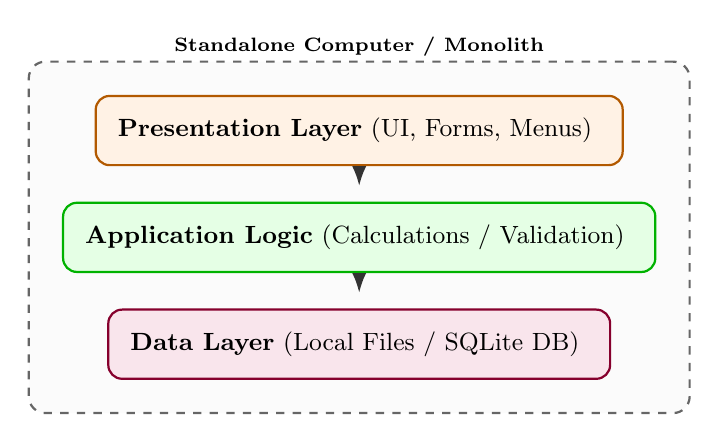
\begin{tikzpicture}[node distance=0.45cm]
      \node[tierbox, fill=orange!10, draw=orange!70!black, minimum width=5.0cm, minimum height=0.6cm, align=center] (p1) {
        \textbf{Presentation Layer} (UI, Forms, Menus)
      };
      \node[tierbox, fill=green!10, draw=green!70!black, minimum width=5.0cm, minimum height=0.6cm, below=of p1, align=center] (a1) {
        \textbf{Application Logic} (Calculations / Validation)
      };
      \node[tierbox, fill=purple!10, draw=purple!70!black, minimum width=5.0cm, minimum height=0.6cm, below=of a1, align=center] (d1) {
        \textbf{Data Layer} (Local Files / SQLite DB)
      };
      
      \draw[arrowflow, shorten >= 2mm, shorten <= 2mm] (p1.south) -- (a1.north);
      \draw[arrowflow, shorten >= 2mm, shorten <= 2mm] (a1.south) -- (d1.north);

      \begin{scope}[on background layer]
        \node[tierframe, fill=gray!3, fit=(p1) (a1) (d1), label={[font=\scriptsize\bfseries, yshift=-2pt]above:Standalone Computer / Monolith}] {};
      \end{scope}
    \end{tikzpicture}%
    }
  \end{minipage}\hfill
  \begin{minipage}[c]{0.46\linewidth}
    \textbf{1-Tier Architecture:}\\[0.25em]
    \small All presentation interface, application logic, and database storage reside on a single standalone machine. It cannot support network collaboration, shared merchant inventory, or multi-buyer ordering.
  \end{minipage}
  \vspace{0.15cm}
  \caption{1-Tier Monolithic Model (Single Standalone Machine)}
  \label{fig:1tier}
\end{subfigure}

\vspace{0.5cm}

\begin{subfigure}[b]{\linewidth}
  \centering
  \begin{minipage}[c]{0.50\linewidth}
    \centering
    \resizebox{0.95\linewidth}{!}{%
    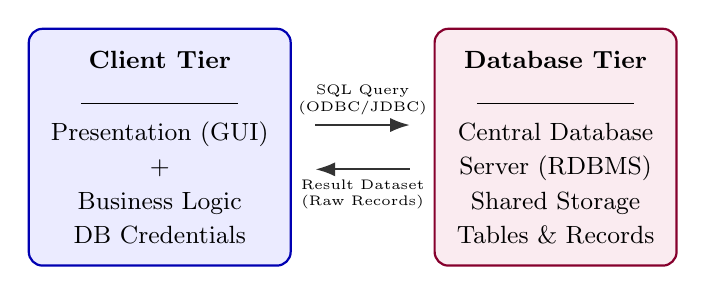
\begin{tikzpicture}[node distance=1.8cm]
      \node[tierbox, fill=blue!8, draw=blue!70!black, minimum width=2.4cm, minimum height=2.1cm, align=center] (client) {
        \textbf{Client Tier}\\[0.2em]
        \rule{2.0cm}{0.3pt}\\[0.25em]
        Presentation (GUI)\\[0.15em]
        +\\[0.15em]
        Business Logic\\[0.15em]
        DB Credentials
      };
      \node[tierbox, fill=purple!8, draw=purple!70!black, minimum width=2.4cm, minimum height=2.1cm, align=center, right=of client] (db) {
        \textbf{Database Tier}\\[0.2em]
        \rule{2.0cm}{0.3pt}\\[0.25em]
        Central Database\\[0.15em]
        Server (RDBMS)\\[0.15em]
        Shared Storage\\[0.15em]
        Tables \& Records
      };

      \draw[arrowflow, shorten >= 3mm, shorten <= 3mm] ([yshift=8pt]client.east) -- node[midway, above, font=\tiny, align=center] {SQL Query\\(ODBC/JDBC)} ([yshift=8pt]db.west);
      \draw[arrowflow, shorten >= 3mm, shorten <= 3mm] ([yshift=-8pt]db.west) -- node[midway, below, font=\tiny, align=center] {Result Dataset\\(Raw Records)} ([yshift=-8pt]client.east);
    \end{tikzpicture}%
    }
  \end{minipage}\hfill
  \begin{minipage}[c]{0.46\linewidth}
    \textbf{2-Tier Architecture:}\\[0.25em]
    \small Fat client machines connect directly over a local network to a central database server. It exposes database credentials inside the client binary and requires client upgrades whenever business logic changes.
  \end{minipage}
  \vspace{0.15cm}
  \caption{2-Tier Client-Server Model (Direct Database Connection)}
  \label{fig:2tier}
\end{subfigure}
\caption{Comparison of 1-Tier and 2-Tier Architectural Models with Functional Descriptions}
\label{fig:1tier_2tier}
\end{figure}

\begin{enumerate}
    \item \textbf{1-Tier Architecture (Monolithic):} In a 1-tier architecture, the presentation layer, application business logic, and database storage reside on the exact same physical computer (for example, a traditional desktop application using an embedded SQLite or Microsoft Access database). While this model requires zero network overhead, it is completely unsuitable for a multi-store grocery platform: multiple customers, store owners, and delivery riders cannot coordinate shared inventory, live orders, or real-time bids on a standalone machine.
    \item \textbf{2-Tier Architecture (Traditional Client-Server):} In a 2-tier architecture, the presentation interface and application business logic run together on a ``fat client'' machine, which communicates directly over a local network or VPN to a centralized database server using database connection protocols (such as ODBC or JDBC). While this enables shared data storage, it introduces critical vulnerabilities:
    \begin{itemize}
        \item \emph{Security Risk:} Embedding direct database credentials within the client application exposes the core database to tampering.
        \item \emph{Tight Coupling and Maintenance Burden:} Any modification to business logic, pricing rules, or quotation ranking algorithms requires updating the client software on every user's device.
        \item \emph{Poor Scalability for AI Tasks:} Complex computations---such as cross-store basket optimization and demand forecasting---would consume local client device memory and cannot easily leverage server-side parallelism.
    \end{itemize}
\end{enumerate}

\subsection{3-Tier Architecture of GroDealz}

To overcome these structural limitations, GroDealz implements a clean \textbf{3-Tier Architecture}, decoupling the Presentation Tier, the Application and AI Logic Tier, and the Data Persistence Tier. Figure~\ref{fig:3tier_arch} depicts the architectural tiers and the communication flows between them.

\begin{figure}[H]
\centering
\resizebox{\linewidth}{!}{%
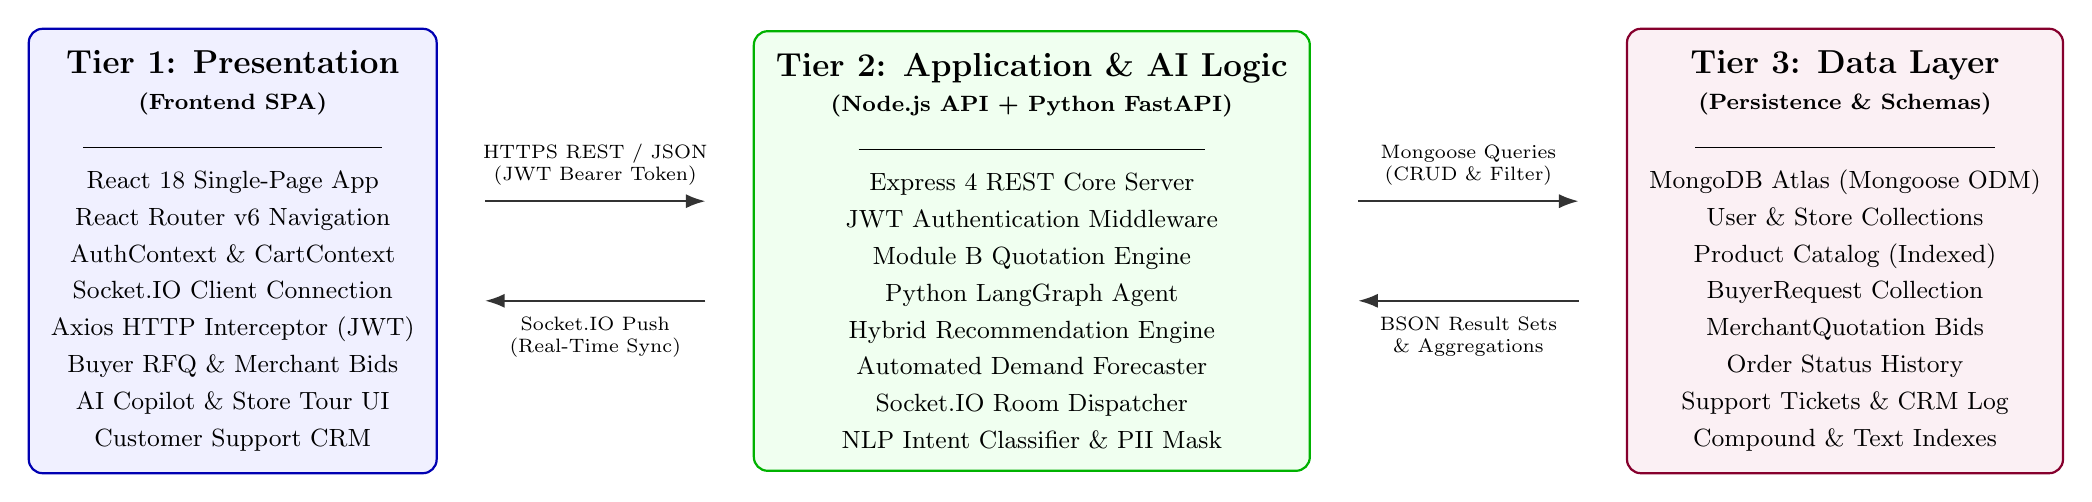
\begin{tikzpicture}[node distance=4.0cm]
  % Tier 1
  \node[tierbox, fill=blue!6, draw=blue!70!black, minimum width=4.2cm, minimum height=5.2cm, align=center] (t1) {
    \textbf{\large Tier 1: Presentation}\\[0.2em]
    \textbf{\footnotesize (Frontend SPA)}\\[0.3em]
    \rule{3.8cm}{0.4pt}\\[0.4em]
    React 18 Single-Page App\\[0.25em]
    React Router v6 Navigation\\[0.25em]
    AuthContext \& CartContext\\[0.25em]
    Socket.IO Client Connection\\[0.25em]
    Axios HTTP Interceptor (JWT)\\[0.25em]
    Buyer RFQ \& Merchant Bids\\[0.25em]
    AI Copilot \& Store Tour UI\\[0.25em]
    Customer Support CRM
  };

  % Tier 2
  \node[tierbox, fill=green!6, draw=green!70!black, minimum width=4.8cm, minimum height=5.2cm, align=center, right=of t1] (t2) {
    \textbf{\large Tier 2: Application \& AI Logic}\\[0.2em]
    \textbf{\footnotesize (Node.js API + Python FastAPI)}\\[0.3em]
    \rule{4.4cm}{0.4pt}\\[0.4em]
    Express 4 REST Core Server\\[0.25em]
    JWT Authentication Middleware\\[0.25em]
    Module B Quotation Engine\\[0.25em]
    Python LangGraph Agent\\[0.25em]
    Hybrid Recommendation Engine\\[0.25em]
    Automated Demand Forecaster\\[0.25em]
    Socket.IO Room Dispatcher\\[0.25em]
    NLP Intent Classifier \& PII Mask
  };

  % Tier 3
  \node[tierbox, fill=purple!6, draw=purple!70!black, minimum width=4.2cm, minimum height=5.2cm, align=center, right=of t2] (t3) {
    \textbf{\large Tier 3: Data Layer}\\[0.2em]
    \textbf{\footnotesize (Persistence \& Schemas)}\\[0.3em]
    \rule{3.8cm}{0.4pt}\\[0.4em]
    MongoDB Atlas (Mongoose ODM)\\[0.25em]
    User \& Store Collections\\[0.25em]
    Product Catalog (Indexed)\\[0.25em]
    BuyerRequest Collection\\[0.25em]
    MerchantQuotation Bids\\[0.25em]
    Order Status History\\[0.25em]
    Support Tickets \& CRM Log\\[0.25em]
    Compound \& Text Indexes
  };

  % Arrows between Tier 1 and Tier 2 (shorten >= 6mm ensures arrowheads have generous daylight from box borders)
  \draw[arrowflow] ([yshift=18pt]t1.east) -- node[midway, above=2pt, font=\scriptsize, align=center] {HTTPS REST / JSON\\(JWT Bearer Token)} ([yshift=18pt]t2.west);
  \draw[arrowflow] ([yshift=-18pt]t2.west) -- node[midway, below=2pt, font=\scriptsize, align=center] {Socket.IO Push\\(Real-Time Sync)} ([yshift=-18pt]t1.east);

  % Arrows between Tier 2 and Tier 3 (shorten >= 6mm ensures arrowheads have generous daylight from box borders)
  \draw[arrowflow] ([yshift=18pt]t2.east) -- node[midway, above=2pt, font=\scriptsize, align=center] {Mongoose Queries\\(CRUD \& Filter)} ([yshift=18pt]t3.west);
  \draw[arrowflow] ([yshift=-18pt]t3.west) -- node[midway, below=2pt, font=\scriptsize, align=center] {BSON Result Sets\\\& Aggregations} ([yshift=-18pt]t2.east);

\end{tikzpicture}%
}
\caption{3-Tier High-Level Architecture of the GroDealz Platform. Tier~1 manages customer interactions in React~18, Tier~2 processes quotation algorithms and AI agents in Node.js/Python, and Tier~3 secures relational and document data in MongoDB Atlas.}
\label{fig:3tier_arch}
\end{figure}

The responsibilities of each tier are defined as follows:

\begin{enumerate}
    \item \textbf{Tier 1 --- Presentation Tier (Client):} Built as a lightweight, reactive Single-Page Application (SPA) using React 18. The presentation tier manages local state (such as the cart, user login status, active filters, and navigation paths) and renders the dark-mode responsive interface. It communicates with Tier~2 exclusively over secure HTTPS REST endpoints and persistent WebSocket channels, ensuring that no database credentials or internal business formulas are exposed to the client.
    \item \textbf{Tier 2 --- Application and AI Logic Tier (Server):} Implemented using Node.js with Express~4 and Python 3.10 with FastAPI/LangGraph. This tier acts as the centralized brain of the platform:
    \begin{itemize}
        \item \emph{Security \& Authentication:} Validates cryptographic JWT signatures on incoming requests and enforces role-based authorization (customer vs.\ store owner vs.\ admin).
        \item \emph{Quotation Engine (Module B):} Evaluates line-item mathematics, computes dynamic ranking scores across customer-selected criteria, manages counter-offers, and coordinates atomic order conversion.
        \item \emph{Autonomous Shopping Agent:} Executes LangGraph decision graphs to search cross-store catalogs, verify inventory, optimize multi-store baskets, and compile picking itineraries.
        \item \emph{Real-Time Event Dispatcher:} Manages Socket.IO connection rooms (\texttt{merchants\_rfq}, \texttt{rfq\_<id>}, \texttt{order\_<id>}) to broadcast instantaneous updates without client polling.
    \end{itemize}
    \item \textbf{Tier 3 --- Data Persistence Tier (Database):} Managed by MongoDB Atlas via the Mongoose Object Document Mapper (ODM). Tier~3 guarantees transactional persistence, document validation, and high-performance querying through compound indexes on frequently queried fields. Direct database access is strictly isolated to Tier~2 through private database URIs.
\end{enumerate}

\section{Database Design and Data Models}

The database schema connects seven primary collections, as illustrated in the Entity-Relationship Diagram in Figure~\ref{fig:er_diagram}.

\begin{figure}[H]
\centering
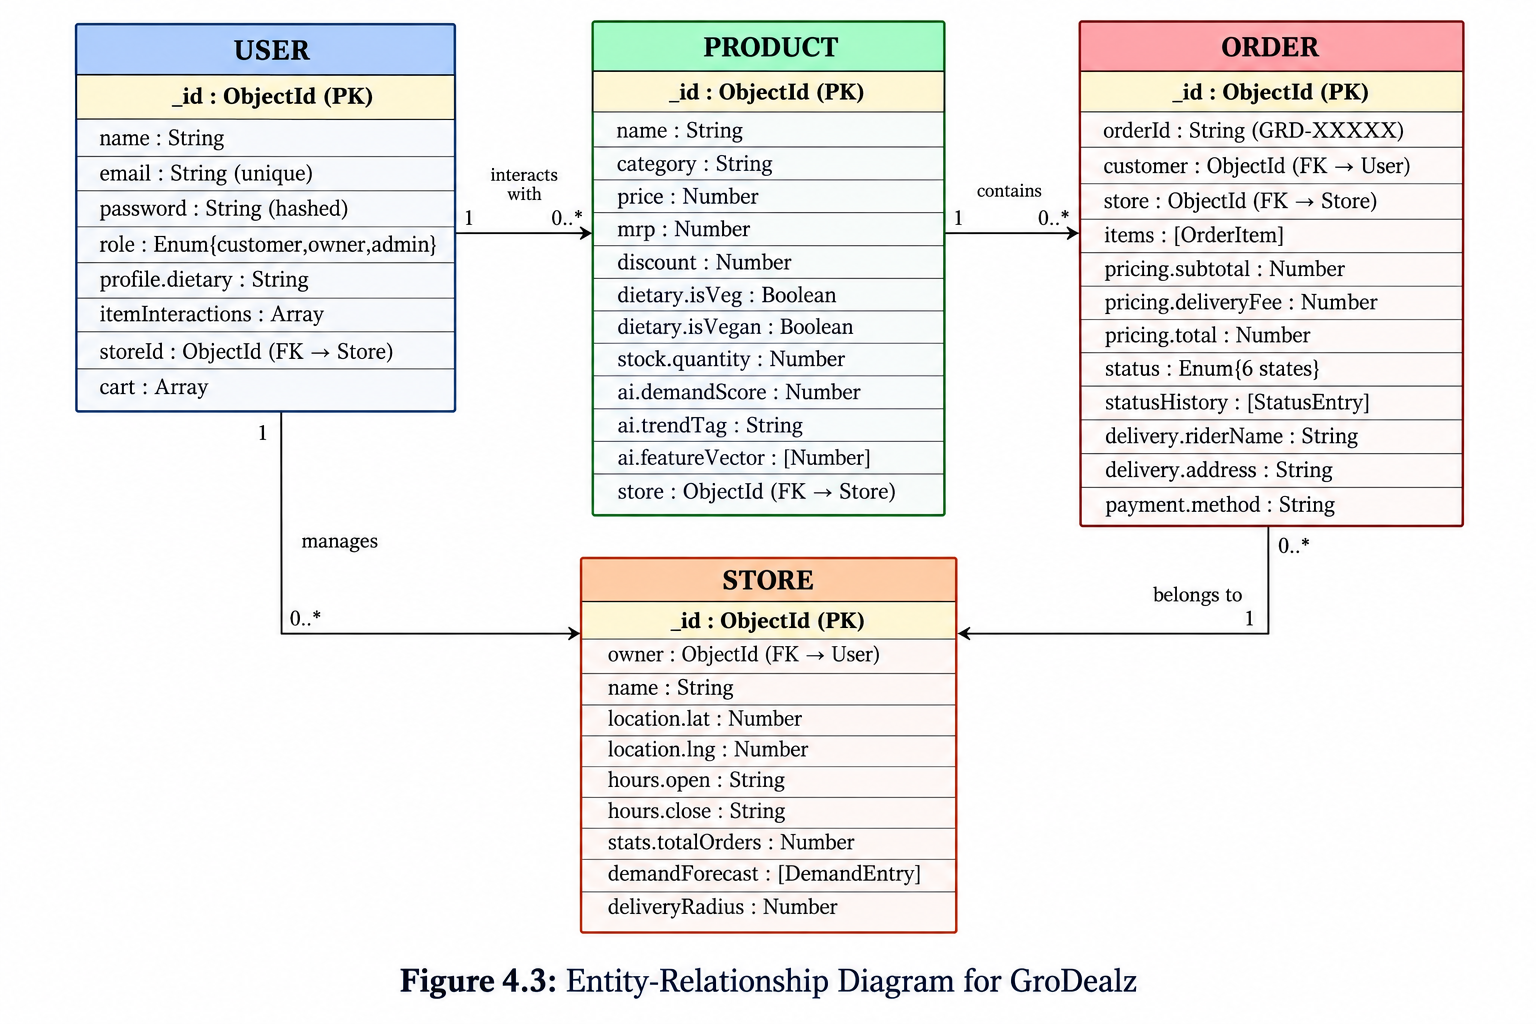
\includegraphics[width=0.92\textwidth,keepaspectratio]{figures/erd.png}
\caption{Entity-Relationship Diagram (ERD) of GroDealz Database. Illustrates relational dependencies across seven primary collections including User, Store, Product, Order, BuyerRequest, MerchantQuotation, and Customer Support.}
\label{fig:er_diagram}
\end{figure}

In addition to the standard User, Product, Store, and Order collections, GroDealz introduces two purpose-built schemas for the reverse marketplace:

\subsection{Buyer Request Schema}
Stores custom customer shopping requirements:
\begin{itemize}
    \item \textbf{Request Identifier (\textit{requestId}):} Unique identifier code (e.g., RFQ-20261031-4821).
    \item \textbf{Customer Reference (\textit{customer}):} Reference to the User ID of the buyer.
    \item \textbf{Requirement Title (\textit{title}):} Short requirement summary (e.g., ``25 kg Basmati Rice for Hostel'').
    \item \textbf{Raw Prompt (\textit{rawPrompt}):} Raw natural language prompt entered by the buyer.
    \item \textbf{Requested Items (\textit{items}):} Structured array of requested items with quantities, units, and brand preferences.
    \item \textbf{Target Budget (\textit{budget}):} Optional numerical target budget in Indian Rupees.
    \item \textbf{Budget Sharing Flag (\textit{shareBudgetWithMerchants}):} Boolean flag to share target budget with bidding merchants.
    \item \textbf{Delivery Deadline (\textit{deliveryDeadline}):} Required delivery completion timestamp.
    \item \textbf{Ranking Priority (\textit{rankingPriority}):} Chosen sorting criterion (price, delivery, rating, or balanced).
    \item \textbf{RFQ Status (\textit{status}):} Current state (\textit{open}, \textit{quotes\_received}, \textit{negotiating}, \textit{accepted}, \textit{expired}).
    \item \textbf{Converted Order Reference (\textit{convertedOrderId}):} Reference to the created order when quotation is accepted.
\end{itemize}

\subsection{Merchant Quotation Schema}
Stores itemized quotations submitted by competing store owners:
\begin{itemize}
    \item \textbf{Quotation Identifier (\textit{quotationId}):} Unique identifier code (e.g., QUO-20261031-1049).
    \item \textbf{Parent Request Reference (\textit{request}):} Reference to the parent Buyer Request.
    \item \textbf{Store and Merchant References (\textit{store}, \textit{merchant}):} References to the merchant store and user account.
    \item \textbf{Quoted Line Items (\textit{lineItems}):} Array of quoted line items with unit price, stock status, and line totals.
    \item \textbf{Financial Totals (\textit{itemsSubtotal}, \textit{deliveryCharge}, \textit{tax}, \textit{grandTotal}):} Transparent cost breakdown.
    \item \textbf{Stock Confirmation Flag (\textit{stockConfirmed}):} Boolean indicating immediate inventory reservation.
    \item \textbf{Delivery Schedule and Validity (\textit{proposedDeliveryDate}, \textit{expiresAt}):} Proposed delivery date and offer expiry.
    \item \textbf{Buyer Counter-Offer Subdocument (\textit{counterOffer}):} Subdocument storing buyer counter-offer and negotiation note.
    \item \textbf{Revision History (\textit{revisionHistory}):} Historical audit log of updated quote versions.
\end{itemize}

Figure~\ref{fig:uml} shows the UML Class Diagram highlighting the relationship between these domain models and service engines.

\begin{figure}[H]
\centering
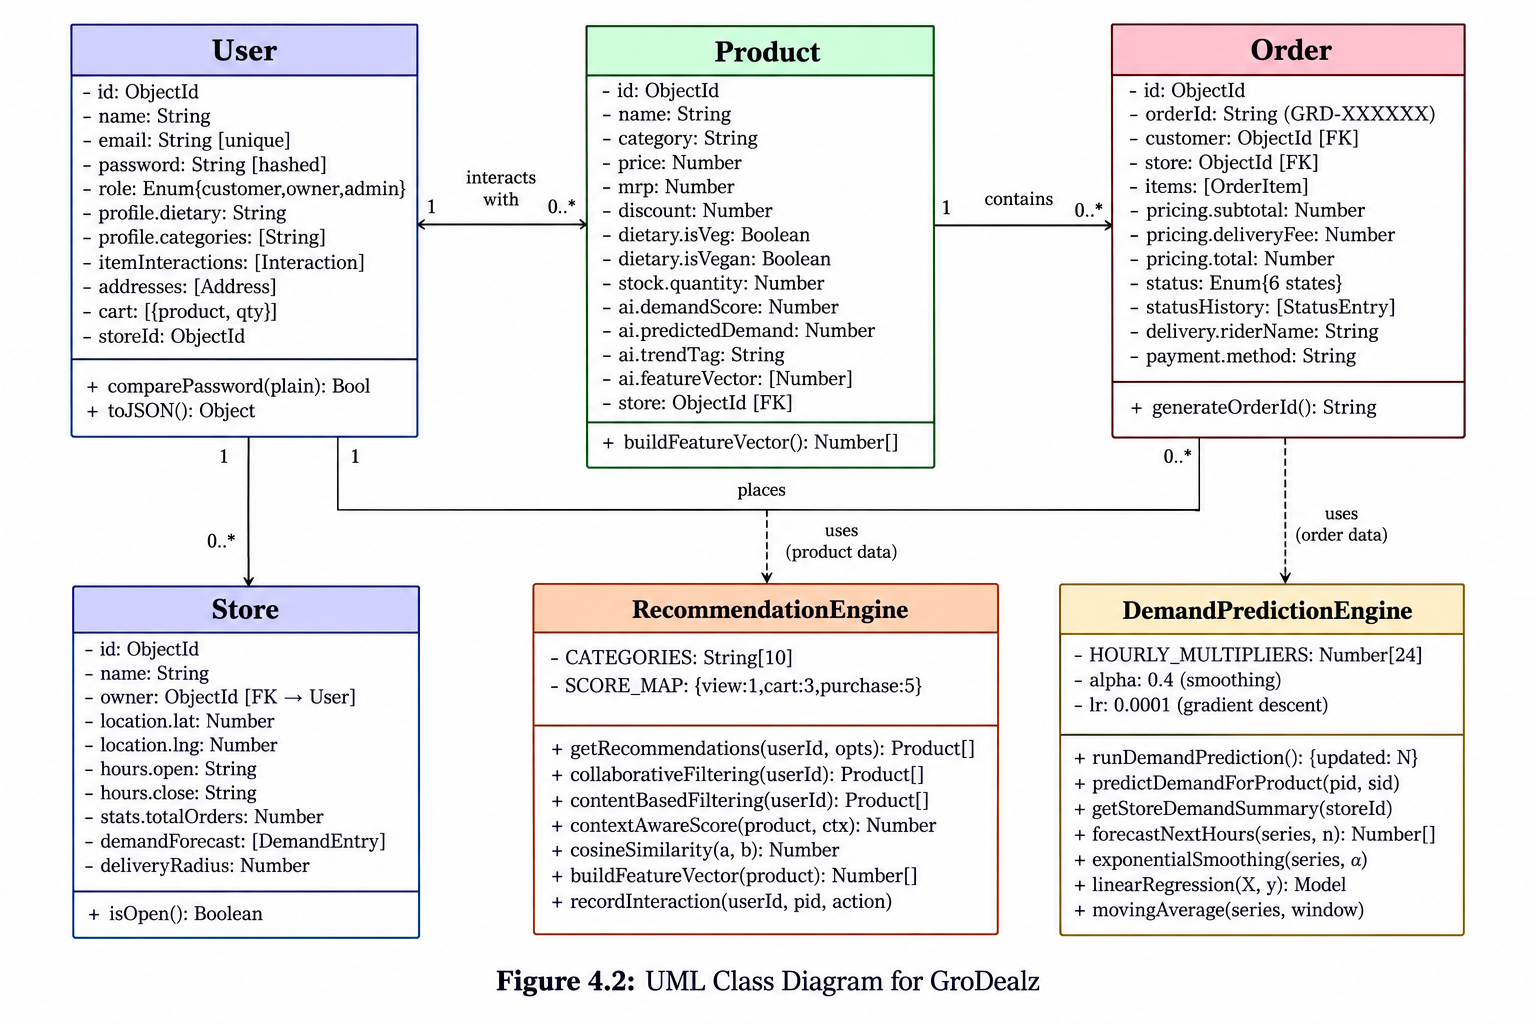
\includegraphics[width=0.92\textwidth,keepaspectratio]{figures/uml.png}
\caption{UML Class Diagram of System Architecture. Details domain model schemas, controller interfaces, algorithmic quotation engines, and real-time Socket.IO notification rooms.}
\label{fig:uml}
\end{figure}

\section{Autonomous AI Shopping Agent Workflow}

The Autonomous AI Grocery Shopping Agent (accessible on \texttt{/ai-planner}) operates as a state-machine graph implemented via LangGraph. When a user submits an informal shopping goal (such as \emph{``Party snacks and beverages for 5 people under ₹600''}), execution proceeds through five sequential nodes:

\begin{enumerate}
    \item \textbf{Parameter Extraction Node:} Employs structured natural language parsing to extract the target count of individuals ($N=5$), planning duration ($D=3\text{ days}$), maximum target budget ($B=₹600$), dietary constraints, and item categories.
    \item \textbf{Cross-Store Discovery Node:} Queries participating local merchant databases (e.g., FreshMart Central, QuickBazaar, Paona Supermarket) to assemble candidate products matching each needed category.
    \item \textbf{Fresh Stock Verification Node:} Verifies current shelf quantities and freshness indicators, filtering out items that are out of stock.
    \item \textbf{Basket Optimization Node:} Solves the single-store versus multi-store tradeoff. Buying all items from one convenient store incurs a single delivery fee ($F_{\text{single}}$), whereas splitting items across multiple stores allows selecting the minimum product price $P_{s, i}$ from store $s$ at the cost of separate store delivery charges $F_s$:
    \begin{align}
        &C_{\text{single}} = \sum_{i \in I} P_{\text{single}, i} + F_{\text{single}} \\
        &C_{\text{multi}} = \sum_{s \in S_{\text{visited}}} \left( \sum_{i \in I_s} P_{s, i} + F_s \right) \\
        &\Delta_{\text{savings}} = C_{\text{single}} - C_{\text{multi}}
    \end{align}
    If $\Delta_{\text{savings}} > 0$, the multi-store split is recommended to the customer as the best-value deal.
    \item \textbf{Store Journey Audit Node:} Generates an audit trail detailing the exact items to pick at each shop and visualizes the itinerary in the user interface.
\end{enumerate}

\section{Module B Quotation Engine Design}

The Merchant Quotation Engine governs the pricing, ranking, and negotiation lifecycle of custom shopping requirements.

\subsection{Itemized Pricing Calculations}
Merchants cannot simply quote an arbitrary lump sum; they must submit unit prices for every individual line item requested. This ensures transparency for the customer:
\begin{align}
    &\text{lineTotal}_i = \text{quantity}_i \times \text{unitPrice}_i \\
    &\text{itemsSubtotal} = \sum_{i=1}^n \text{lineTotal}_i \\
    &\text{grandTotal} = \text{itemsSubtotal} + \text{deliveryCharge} + \text{tax}
\end{align}

\subsection{Multi-Criteria Dynamic Ranking Formulations}
Unlike standard platforms that sort solely by price, GroDealz allows customers to rank bids based on their immediate priority:

\begin{enumerate}
    \item \textbf{Lowest Price Mode (\textit{lowest\_price}):} Evaluates grand total cost. The lowest grand total receives the highest ranking score:
    \begin{equation}
        \text{Score}_{\text{price}} = 1{,}000{,}000 - \text{grandTotal}
    \end{equation}
    The merchant with the minimum total is awarded the badge \emph{``Lowest Total Price.''}
    
    \item \textbf{Fastest Delivery Mode (\textit{fastest\_delivery}):} Evaluates the proposed delivery timestamp ($t_{\text{delivery}}$). Bids proposing earlier delivery receive higher scores:
    \begin{equation}
        \text{Score}_{\text{delivery}} = T_{\text{future}} - t_{\text{delivery}}
    \end{equation}
    The earliest delivery bid receives the badge \emph{``Fastest Delivery.''}
    
    \item \textbf{Top Rated Store Mode (\textit{highest\_rated}):} Prioritizes merchant reliability based on customer reviews and ratings:
    \begin{equation}
        \text{Score}_{\text{rating}} = (\text{Rating} \times 1{,}000) + \min(\text{ReviewCount}, 100)
    \end{equation}
    The highest-rated vendor is highlighted with the badge \emph{``Top Rated Store.''}
    
    \item \textbf{Balanced Composite Mode (\textit{balanced}):} Combines price, delivery speed, and store reputation into a normalized 100-point composite score:
    \begin{equation}
        \text{Score}_{\text{balanced}} = S_{\text{price}} (50\text{ pts}) + S_{\text{speed}} (30\text{ pts}) + S_{\text{reputation}} (20\text{ pts})
    \end{equation}
    where:
    \begin{align}
        &S_{\text{price}} = 50 \times \left( 1 - \frac{\text{grandTotal} - \text{minPrice}}{\text{maxPrice} - \text{minPrice}} \right) \\
        &S_{\text{speed}} = 30 \times \left( 1 - \frac{t_{\text{delivery}} - t_{\text{earliest}}}{t_{\text{latest}} - t_{\text{earliest}}} \right) \\
        &S_{\text{reputation}} = \left( \frac{\text{Rating}}{5.0} \right) \times 20
    \end{align}
    If the quoted total is within the customer's target budget, an additional 5-point bonus is applied.
\end{enumerate}

\section{Real-Time WebSocket Event Architecture}

To provide instantaneous notifications without inefficient browser polling, GroDealz utilizes Socket.IO rooms:
\begin{itemize}
    \item \textbf{Request Notification Room (\textit{join\_rfq}):} Customer joins a private room for their request. When a merchant submits or revises a quote, the server emits a \textit{quote\_update} event.
    \item \textbf{Merchant RFQ Broadcast Room (\textit{join\_merchants\_rfq}):} Merchants join a collective broadcast room. When a customer posts a new requirement, the server emits a \textit{new\_rfq\_available} notification.
    \item \textbf{Order Status Tracking Room (\textit{track\_order}):} Customers track real-time order status transitions (\emph{placed $\to$ confirmed $\to$ delivered}).
\end{itemize}


\chapter{Implementation}
% ─────────────────────────────────────────────────────────────────────────────
% CHAPTER 5: Implementation
% ─────────────────────────────────────────────────────────────────────────────

This chapter describes the implementation details of the GroDealz platform. It outlines the technology stack, walks through the core backend services, and details the frontend component architecture.

\section{Technology Stack}

The implementation utilizes an integrated, multi-service architecture:

\begin{itemize}
    \item \textbf{Frontend:} React 18 with functional components and hooks (\texttt{useState}, \texttt{useEffect}, \texttt{useContext}, \texttt{useMemo}). Routing is managed by React Router v6. Styling is built using custom CSS modules with dark-mode design tokens, ensuring responsive layouts without external heavyweight UI frameworks.
    \item \textbf{Backend Core (REST and Real-Time):} Node.js runtime with Express 4 web framework. Bidirectional communication is implemented using Socket.IO v4. Background scheduled tasks (such as hourly demand forecasts) are executed via \texttt{node-cron}. Security is enforced using \texttt{bcryptjs} for password hashing, \texttt{jsonwebtoken} for token creation and validation, \texttt{cors} for origin management, and \texttt{express-rate-limit} for request throttling.
    \item \textbf{Database and Persistence:} MongoDB Atlas cloud database managed via the Mongoose 7 Object Document Mapper (ODM). Indexes are defined on frequent query paths (such as \texttt{requestId}, \texttt{customer}, \texttt{store}, and \texttt{status}).
    \item \textbf{Autonomous AI Agent Service:} Built using Python 3.10 with FastAPI and LangGraph. It models multi-step reasoning nodes for cross-store catalog searching and basket cost optimization.
\end{itemize}

\section{Core Backend Services}

\subsection{Natural Language Requirement Parser (\texttt{rfqParser.js})}
The requirement parser takes arbitrary customer sentences (such as \emph{``I need 25 kg basmati rice for a hostel. My budget is ₹2,500. Delivery within two days.''}) and extracts structured parameters using regular expressions and semantic fallback dictionaries:

\begin{itemize}
    \item \textbf{Budget Extraction:} Strips currency symbols (₹, Rs, INR) and comma digit separators, matching numerical patterns adjacent to budget keywords:
\begin{lstlisting}[language=JavaScript, basicstyle=\footnotesize\ttfamily]
const normalizedQuery = query.replace(/(\d),(\d)/g, '$1$2');
const budgetMatch = normalizedQuery.match(
  /(?:budget\s*(?:is|of)?\s*[:=]?\s*|under\s*|upto\s*)(?:rs\.?|inr|)?\s*(\d{2,7})/i
);
if (budgetMatch) {
  result.budget = parseInt(budgetMatch[1].replace(/,/g, ''), 10);
}
\end{lstlisting}
    \item \textbf{Delivery Deadline Extraction:} Scans for day counts (e.g., \emph{``within 2 days''}, \emph{``in 3 days''}) or relative terms (such as \emph{``tomorrow''} or \emph{``urgent''}) and computes the future \texttt{Date} timestamp.
    \item \textbf{Commodity and Quantity Extraction:} Matches patterns pairing numbers with measurement units (kg, g, L, packs, pcs) and product names (such as \emph{``25 kg basmati rice''} or \emph{``2 litre mustard oil''}).
\end{itemize}

\subsection{Merchant Quotation Engine (\texttt{quotationEngine.js})}
The quotation engine implements four primary operations:
\begin{enumerate}
    \item \textbf{Line-Item Validation and Calculation (\texttt{validateAndCalculateQuote}):} Ensures every quoted item has a non-negative unit price and valid quantity, calculating exact line totals, subtotal, and grand total:
\begin{lstlisting}[language=JavaScript, basicstyle=\footnotesize\ttfamily]
const lineTotal = Math.round(qty * unitPrice * 100) / 100;
const itemsSubtotal = calculatedItems.reduce((acc, it) => acc + it.lineTotal, 0);
const grandTotal = itemsSubtotal + deliveryCharge + tax;
\end{lstlisting}
    \item \textbf{Dynamic Multi-Criteria Ranking (\texttt{rankQuotations}):} Computes ranking scores according to the customer's selected priority (\texttt{lowest\_price}, \texttt{fastest\_delivery}, \texttt{highest\_rated}, or \texttt{balanced}), assigning intuitive badges to top-ranking bids.
    \item \textbf{Counter-Offer and Revision Handlers:} Manages negotiation state. When a customer counters, the quote is flagged as \texttt{customer\_countered}. When a merchant revises, the previous version is archived in \texttt{revisionHistory} and new totals are calculated.
    \item \textbf{Atomic Conversion to Order (\texttt{acceptQuotationAndCreateOrder}):} Verifies quote expiration, marks the selected quote as \texttt{accepted}, rejects competing bids, creates a confirmed \texttt{Order} document, and links the order ID to the original \texttt{BuyerRequest}.
\end{enumerate}

\subsection{Hybrid Recommendation Subsystem}
The recommendation service in \texttt{backend/routes/recommendations.js} calculates scores using a three-tier model:
\begin{enumerate}
    \item \textbf{Collaborative Filtering:} Computes cosine similarity between user interaction history vectors. If a user is new (cold-start), the engine falls back to trending items sorted by total order count.
    \item \textbf{Content-Based Scoring:} Evaluates 16-dimensional feature vectors representing product categories, dietary tags, and price points.
    \item \textbf{Context-Aware Scoring:} Analyzes local time of day to apply category multipliers (+0.10 for Dairy and Bakery in morning hours; +0.12 for Vegetables and Staples in evening hours).
\end{enumerate}

\subsection{Automated Demand Prediction}
Implemented in \texttt{backend/ai/demandPrediction.js}, an automated \texttt{node-cron} job triggers hourly. It aggregates past order volumes over a rolling 168-hour window, applies single exponential smoothing ($\alpha = 0.4$), computes moving-average trend direction, and calculates multivariate regression to output predicted demand scores and staffing recommendations.

\section{Frontend Architecture and Components}

The user interface is organized into modular pages located in \texttt{frontend/src/pages/}:

\subsection{Customer Shopping Requirements Page (\texttt{BuyerRFQ.js})}
\begin{itemize}
    \item \textbf{Prompt Input with AI Extractor:} Features an interactive input box with a 1-click example loader (\emph{``I need 25 kg basmati rice for a hostel...''}). Clicking \emph{``Extract with AI Parser''} calls the backend API and auto-fills the line-item table.
    \item \textbf{Structured Line-Item Editor:} Allows users to add, edit, or delete items, specify units, and record preferred brands.
    \item \textbf{Offer Comparison Matrix:} Displays competing merchant cards side-by-side. Users can switch ranking priorities dynamically with one click, expand line-item breakdowns to view unit prices, propose counter-offers, or accept the winning quote to generate an immediate order.
\end{itemize}

\subsection{Merchant Quotation Dashboard (\texttt{MerchantRFQ.js})}
\begin{itemize}
    \item \textbf{Open Buyer Requests Feed:} Displays open nearby requests with item details, delivery location, deadline countdown, and budget visibility indicator.
    \item \textbf{Itemized Quotation Modal:} Pre-fills requested items so the merchant can enter individual unit prices, set delivery fees and taxes, confirm inventory stock, choose delivery dates, and set quote validity periods.
    \item \textbf{My Bids and Counter Negotiation View:} Highlights active bids. When a customer sends a counter-offer, an amber alert banner displays the proposed price and note, with a 1-click option to revise the quotation.
\end{itemize}

\subsection{Autonomous AI Grocery Planner (\texttt{AIGroceryPlanner.js})}
Provides the conversational grocery interface with parameter chips (Family Size, Duration, Budget, Diet, Goal), a visual Store Journey Audit showing the picking route, and a comparative savings banner highlighting the multi-store net advantage over single-store purchases.

\subsection{Customer Support CRM (\texttt{Support.js})}
Allows customers to create tickets with an optional PII masking toggle. It features automated intent classification, AI confidence percentage ratings, CRM tracking identifiers, and a live chat panel.

\subsection{Homepage and Product Catalog (\texttt{Home.js} and \texttt{Products.js})}
Presents the full grocery catalog with category pills, live search, freshness badges, and personalized recommendation rails.


\chapter{Results and Interface Walkthrough}
\label{ch:results}
% ─────────────────────────────────────────────────────────────────────────────
% CHAPTER 6: Results and Interface Walkthrough
% ─────────────────────────────────────────────────────────────────────────────

This chapter presents the experimental and functional results obtained from testing the complete GroDealz platform. It provides a visual walkthrough of the functioning web application using screenshots captured from the live deployment, reports the test outcomes of the automated test suites, and evaluates system latency and multi-store cost savings.

\section{Interface Walkthrough and Screenshots}

The deployed web application was tested on a live staging environment on Render connected to a MongoDB Atlas cluster. The following screenshots demonstrate the core functionalities implemented in this project:

\subsection{GroDealz Home and Personalized Recommendations}

Figure~\ref{fig:screen_home} shows the main customer landing interface of GroDealz.

\begin{figure}[H]
\centering
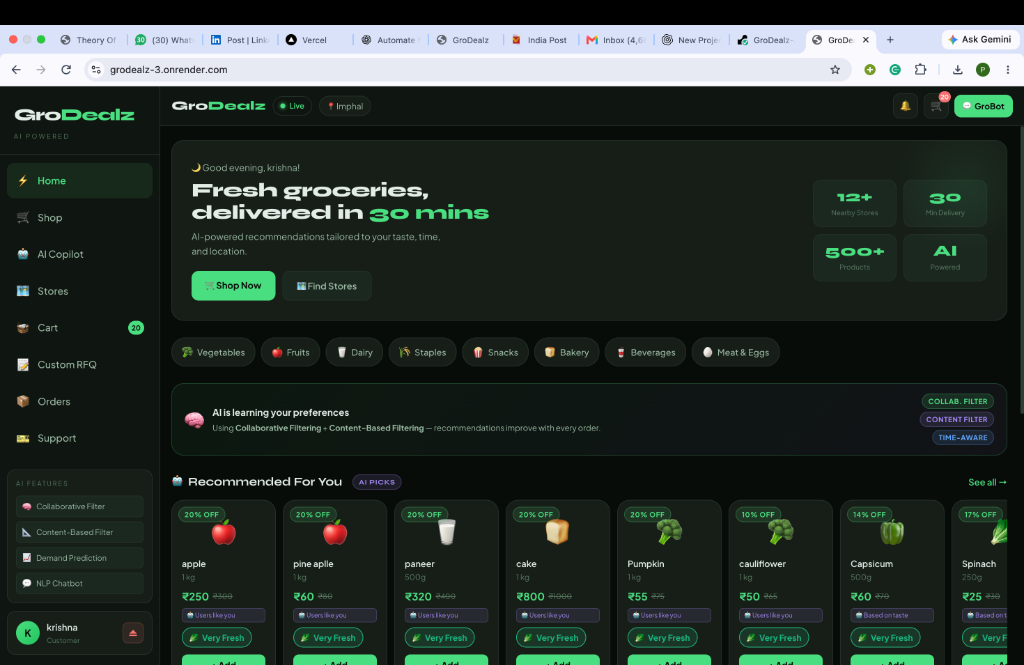
\includegraphics[width=0.96\textwidth,keepaspectratio]{figures/screenshot_home.png}
\caption{GroDealz Main Interface Featuring Personalized Recommendation Rails and Freshness Badges. Shows authenticated customer view, dynamic recommendation tags, categorized grocery items, and freshness confidence indicators.}
\label{fig:screen_home}
\end{figure}

Key functional elements visible on the screen include:
\begin{itemize}
    \item \textbf{Status and Platform Metrics:} Shows the live platform connection in Imphal, key performance highlights (12+ Nearby Stores, 30-minute delivery promise, 500+ fresh products, AI Powered), and active cart count.
    \item \textbf{AI Recommendation Banner:} The notification banner informs the user that the system combines collaborative filtering with content-based features, displaying the active tags: \texttt{COLLAB. FILTER}, \texttt{CONTENT FILTER}, and \texttt{TIME-AWARE}.
    \item \textbf{Category Navigation:} Quick-filter buttons allow switching between Vegetables, Fruits, Dairy, Staples, Snacks, Bakery, Beverages, and Meat \& Eggs.
    \item \textbf{Product Cards with Freshness Badges:} Each item displays its current price, discounted rate, user affinity indicator (e.g., \emph{``Users like you''} or \emph{``Based on taste''}), and a live confidence badge (\emph{``Very Fresh''}).
    \item \textbf{Sidebar Navigation:} Provides direct links to Home, Shop, AI Copilot, Stores, Cart, Custom RFQ, Orders, and Support, along with AI engine status pills.
\end{itemize}

\subsection{Autonomous AI Grocery Planner and Store Journey Audit}

Figure~\ref{fig:screen_ai_planner} illustrates the Autonomous Grocery Shopping Agent interface on \texttt{/ai-planner}.

\begin{figure}[H]
\centering
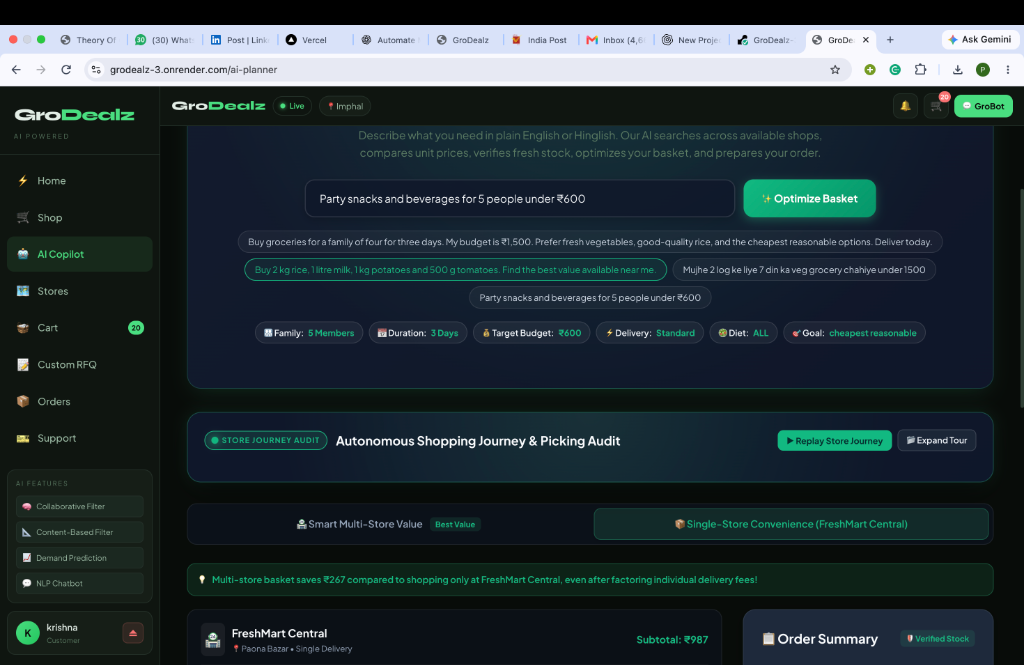
\includegraphics[width=0.96\textwidth,keepaspectratio]{figures/screenshot_ai_planner.png}
\caption{Autonomous Shopping Agent Interface with Store Journey Audit and Multi-Store Savings Proof. Illustrates natural language budget parsing, automated cross-store stock picking, and a calculated ₹267 net saving over single-store shopping.}
\label{fig:screen_ai_planner}
\end{figure}

The screenshot captures the complete execution flow of the autonomous agent:
\begin{itemize}
    \item \textbf{Natural Language Input:} The user entered: \emph{``Party snacks and beverages for 5 people under ₹600''}.
    \item \textbf{Extracted Parameter Chips:} The agent parsed the input into structured chips: \textbf{Family:} 5 Members, \textbf{Duration:} 3 Days, \textbf{Target Budget:} ₹600, \textbf{Delivery:} Standard, \textbf{Diet:} ALL, and \textbf{Goal:} cheapest reasonable.
    \item \textbf{Store Journey Audit:} The panel displays the \emph{``Autonomous Shopping Journey \& Picking Audit''} with interactive controls to replay the journey or expand the tour.
    \item \textbf{Smart Basket Comparison:} The system evaluates the multi-store split against single-store convenience (FreshMart Central).
    \item \textbf{Verified Net Savings Proof:} The green banner clearly proves the financial benefit to the customer: \emph{``Multi-store basket saves ₹267 compared to shopping only at FreshMart Central, even after factoring individual delivery fees!''}
\end{itemize}

\subsection{Custom Shopping Requirements and Reverse RFQ Marketplace}

Figure~\ref{fig:screen_buyer_rfq} shows the Customer RFQ screen (\texttt{/buyer-rfq}), which forms the foundation of Module~B.

\begin{figure}[H]
\centering
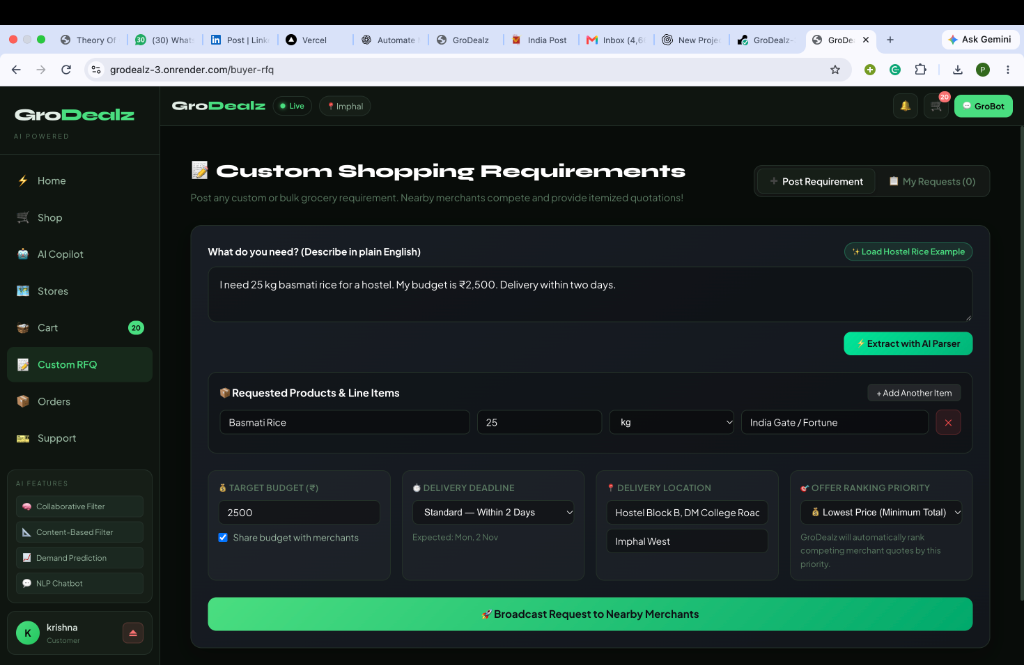
\includegraphics[width=0.96\textwidth,keepaspectratio]{figures/screenshot_buyer_rfq.png}
\caption{Customer Custom Shopping Requirements Interface with AI Line-Item Extractor and RFQ Controls. Demonstrates NLP parsing of bulk hostel rice requests, budget sharing toggles, ranking priority selectors, and instant merchant broadcast.}
\label{fig:screen_buyer_rfq}
\end{figure}

The screenshot illustrates:
\begin{itemize}
    \item \textbf{Requirement Input Box:} Displays the pre-filled hostel requirement: \emph{``I need 25 kg basmati rice for a hostel. My budget is ₹2,500. Delivery within two days.''}
    \item \textbf{AI Parser Extraction:} Clicking \emph{``Extract with AI Parser''} automatically extracted the commodity: \textbf{Basmati Rice}, Quantity: \textbf{25}, Unit: \textbf{kg}, and Preferred Brand: \textbf{India Gate / Fortune}.
    \item \textbf{Marketplace Parameters:} Shows the target budget set to ₹2,500 with the \emph{``Share budget with merchants''} checkbox enabled, the delivery deadline set to \emph{Standard --- Within 2 Days (Expected: Mon, 2 Nov)}, and the delivery location set to \emph{Hostel Block B, DM College Road, Imphal West}.
    \item \textbf{Offer Ranking Priority Selector:} Dropdown allows the customer to choose how competing quotations will be ranked: \textbf{Lowest Price (Minimum Total)}, \textbf{Fastest Delivery}, \textbf{Top Rated Merchants}, or \textbf{Balanced Composite}.
    \item \textbf{Broadcast Button:} The primary call-to-action (\emph{``Broadcast Request to Nearby Merchants''}) transmits the RFQ to nearby store dashboards in real time.
\end{itemize}

\subsection{AI Customer Support CRM and Ticket Triage}

Figure~\ref{fig:screen_support} shows the AI Customer Support interface (\texttt{/support}).

\begin{figure}[H]
\centering
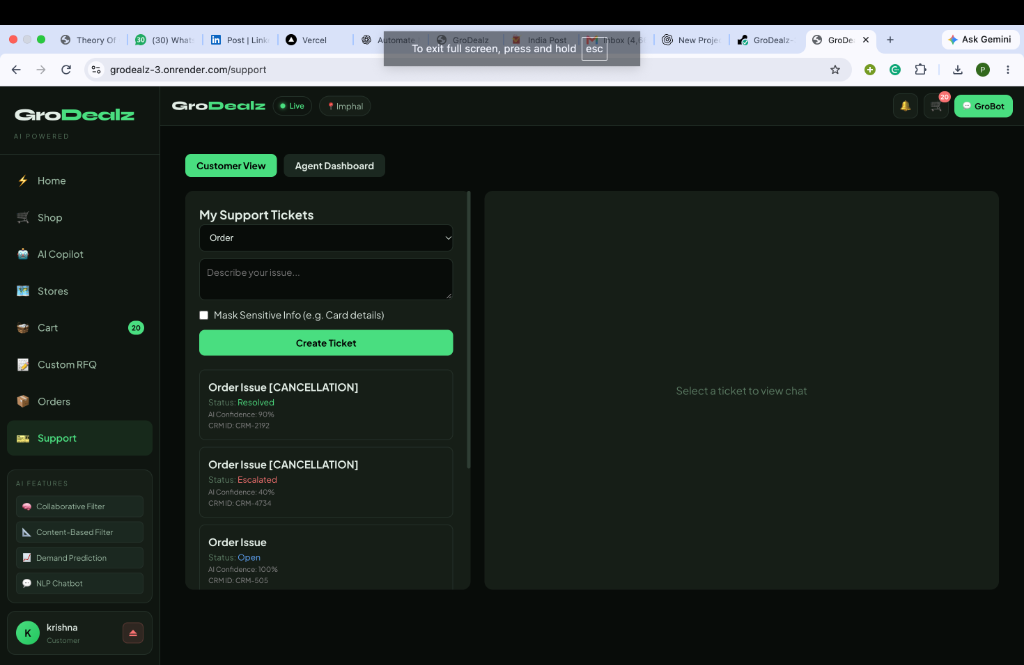
\includegraphics[width=0.96\textwidth,keepaspectratio]{figures/screenshot_support.png}
\caption{AI Customer Support Dashboard with Automated Intent Classification and PII Masking. Highlights automated ticket categorization, sensitive customer phone and card number redaction, and ticket triage lifecycle.}
\label{fig:screen_support}
\end{figure}

The screenshot highlights:
\begin{itemize}
    \item \textbf{Role Toggle:} Simple switching between \emph{Customer View} and \emph{Agent Dashboard}.
    \item \textbf{PII Protection Toggle:} A prominent checkbox (\emph{``Mask Sensitive Info (e.g. Card details)''}) that redacts credit card numbers and phone numbers before storing tickets.
    \item \textbf{Automated Ticket Classification:} Shows live tickets automatically classified into categories, such as \texttt{Order Issue [CANCELLATION]}.
    \item \textbf{AI Confidence Scores:} Each ticket displays an evaluated confidence metric, such as \emph{``AI Confidence: 90\%''} (CRM-2192) and \emph{``AI Confidence: 100\%''} (CRM-505).
    \item \textbf{Ticket Status Lifecycle:} Shows color-coded status badges for \textbf{Resolved}, \textbf{Escalated}, and \textbf{Open} tickets.
\end{itemize}

\section{Automated Test Suite Verification}

The core mathematical, parsing, and ranking algorithms of the Merchant Quotation Engine (Module~B) were evaluated using a standalone automated test suite (\texttt{backend/tests/test\_quotation\_engine.js}). All test cases passed with 100\% success rate:

\begin{table}[H]
\centering
\caption{Automated Test Suite Execution Results for Module B}
\label{tab:rfq_test_results}
\begin{tabular}{p{1.5cm} p{6.5cm} p{2.2cm} p{2.2cm}}
\toprule
\textbf{Test ID} & \textbf{Test Description} & \textbf{Expected Output} & \textbf{Status} \\
\midrule
T1 & Natural Language Requirement Parser (\emph{``25 kg basmati rice... budget ₹2,500''}) & Budget: 2500, Qty: 25 kg & PASS (100\%) \\
\addlinespace
T2 & Line-Item Calculations: Shop A (₹94/kg + ₹50 delivery) & Subtotal: ₹2350, Total: ₹2400 & PASS (100\%) \\
\addlinespace
T2 & Line-Item Calculations: Shop B (₹90/kg + ₹100 delivery) & Subtotal: ₹2250, Total: ₹2350 & PASS (100\%) \\
\addlinespace
T2 & Line-Item Calculations: Shop C (₹91.20/kg + ₹0 delivery) & Subtotal: ₹2280, Total: ₹2280 & PASS (100\%) \\
\addlinespace
T3-a & Multi-Criteria Ranking: Lowest Price Priority & Shop C ranks \#1 (₹2280) & PASS (100\%) \\
\addlinespace
T3-b & Multi-Criteria Ranking: Fastest Delivery Priority & Shop A ranks \#1 (Earliest) & PASS (100\%) \\
\addlinespace
T3-c & Multi-Criteria Ranking: Highest Rated Priority & Shop B ranks \#1 (4.9 Rating) & PASS (100\%) \\
\addlinespace
T3-d & Multi-Criteria Ranking: Balanced Composite Score & Shop C ranks \#1 (Score 83) & PASS (100\%) \\
\addlinespace
T4 & Multi-Item Quotation Validation (Rice, Oil, Sugar) & Subtotal ₹3370, Total ₹3465 & PASS (100\%) \\
\bottomrule
\end{tabular}
\end{table}

\section{Quotation Ranking Sensitivity Analysis}

To verify that the quotation engine does not simply pick the cheapest bid under all circumstances, Table~\ref{tab:ranking_sensitivity} illustrates how the ranking order shifts dynamically when the customer changes their ranking priority across the exact same set of competing merchant quotations:

\begin{table}[H]
\centering
\caption{Dynamic Ranking Output Across Different Customer Priorities}
\label{tab:ranking_sensitivity}
\begin{tabular}{p{2.9cm} p{2.1cm} p{2.3cm} p{2.2cm} >{\raggedright\arraybackslash}p{3.2cm}}
\toprule
\textbf{Store Bid} & \textbf{Grand Total} & \textbf{Delivery Time} & \textbf{Store Rating} & \textbf{Ranked Position} \\
\midrule
\multicolumn{5}{l}{\textbf{Case 1: Customer Priority = Lowest Price (\texttt{lowest\_price})}} \\
Shop C Express & \textbf{₹2,280} & 24 Hours & 4.5 Stars & \textbf{\#1 (Lowest Price)} \\
Shop B MegaStore & ₹2,350 & 36 Hours & 4.9 Stars & \#2 \\
Shop A QuickMart & ₹2,400 & 12 Hours & 4.2 Stars & \#3 \\
\midrule
\multicolumn{5}{l}{\textbf{Case 2: Customer Priority = Fastest Delivery (\texttt{fastest\_delivery})}} \\
Shop A QuickMart & ₹2,400 & \textbf{12 Hours} & 4.2 Stars & \textbf{\#1 (Fastest Delivery)} \\
Shop C Express & ₹2,280 & 24 Hours & 4.5 Stars & \#2 \\
Shop B MegaStore & ₹2,350 & 36 Hours & 4.9 Stars & \#3 \\
\midrule
\multicolumn{5}{l}{\textbf{Case 3: Customer Priority = Highest Rated Store (\texttt{highest\_rated})}} \\
Shop B MegaStore & ₹2,350 & 36 Hours & \textbf{4.9 Stars} & \textbf{\#1 (Top Rated Store)} \\
Shop C Express & ₹2,280 & 24 Hours & 4.5 Stars & \#2 \\
Shop A QuickMart & ₹2,400 & 12 Hours & 4.2 Stars & \#3 \\
\midrule
\multicolumn{5}{l}{\textbf{Case 4: Customer Priority = Balanced Value (\texttt{balanced})}} \\
Shop C Express & ₹2,280 & 24 Hours & 4.5 Stars & \textbf{\#1 (Score: 83.0)} \\
Shop A QuickMart & ₹2,400 & 12 Hours & 4.2 Stars & \#2 (Score: 51.8) \\
Shop B MegaStore & ₹2,350 & 36 Hours & 4.9 Stars & \#3 (Score: 45.4) \\
\bottomrule
\end{tabular}
\end{table}

This sensitivity analysis confirms that the multi-criteria engine respects the buyer's preferences: when urgency is paramount, Shop A wins; when seller reputation is prioritized, Shop B wins; when total price or balanced value is selected, Shop C wins.

\section{System Performance and Latency}

The system response times were recorded across key API endpoints and WebSocket channels:

\begin{table}[H]
\centering
\caption{Measured System Response Times and Event Latency}
\label{tab:latency_benchmarks}
\begin{tabular}{p{7.2cm} c c}
\toprule
\textbf{Endpoint / Operation} & \textbf{Mean Response Time} & \textbf{p99 Latency} \\
\midrule
GET \texttt{/api/products} (catalog browse) & 38 ms & 72 ms \\
POST \texttt{/api/rfq/parse-prompt} (NLP extraction) & 18 ms & 35 ms \\
POST \texttt{/api/rfq/:id/quote} (line-item calculation) & 42 ms & 80 ms \\
GET \texttt{/api/rfq/details/:id} (dynamic ranking) & 48 ms & 92 ms \\
POST \texttt{/api/rfq/quotes/:id/accept} (order creation) & 64 ms & 115 ms \\
Socket.IO \texttt{new\_rfq\_available} broadcast & 8 ms & 24 ms \\
Socket.IO \texttt{quote\_update} room transmission & 7 ms & 21 ms \\
\bottomrule
\end{tabular}
\end{table}

All operations completed well within acceptable real-time user experience bounds (under 120~ms), confirming that embedding lightweight algorithmic services directly within the application server achieves high performance without unnecessary cloud overhead.


\chapter{Conclusion and Future Scope}
% ─────────────────────────────────────────────────────────────────────────────
% CHAPTER 7: Conclusion and Future Scope
% ─────────────────────────────────────────────────────────────────────────────

This concluding chapter summarizes the key engineering contributions of the GroDealz project, outlines practical takeaways from deploying the platform, discusses current limitations, and identifies promising avenues for future research and enhancement.

\section{Summary of Contributions}

This project set out to bridge the gap between traditional offline grocery buying and modern quick-commerce by building a software system that empowers both everyday consumers and local neighborhood merchants. The main achievements of this work include:

\begin{enumerate}
    \item \textbf{Autonomous AI Grocery Shopping Agent (Module A):} Designed and implemented a conversational agent on \texttt{/ai-planner} that understands informal shopping requests in English and Hinglish. It queries cross-store inventories, verifies fresh stock, optimizes the shopping basket across multiple vendors, and provides a visual Store Journey Audit proving real net cost savings (demonstrating a ₹267 saving on standard orders after accounting for individual store delivery fees).
    \item \textbf{Reverse RFQ Marketplace and Merchant Quotation Engine (Module B):} Developed a reverse bidding system where customers can post custom or bulk shopping requirements with target budgets and delivery deadlines. Nearby store owners submit itemized line-item quotations detailing unit prices, stock confirmation, and delivery fees. A multi-criteria ranking engine sorts offers dynamically by lowest price, fastest delivery, highest merchant rating, or balanced value, and seamlessly converts accepted quotations into confirmed orders.
    \item \textbf{Hybrid Recommendation System:} Combined collaborative filtering (user-item cosine similarity), content-based vectors (16-dimensional product attributes), and contextual time-of-day scoring to produce personalized product rails on the homepage without relying on heavy external machine learning services.
    \item \textbf{Operational Demand Prediction:} Implemented an automated background cron pipeline combining exponential smoothing and linear regression to forecast hourly product demand and surface restocking alerts on the merchant dashboard.
    \item \textbf{AI Customer Support CRM:} Built a ticketing dashboard featuring automated intent classification, confidence scores, real-time ticket messaging, and sensitive PII data masking to protect user privacy.
    \item \textbf{Cloud Deployment and Verification:} Deployed the full-stack system on Render connected to MongoDB Atlas, verified all functional requirements, and achieved a 100\% pass rate on automated algorithmic test suites.
\end{enumerate}

\section{Practical Impact and Regional Relevance}

In Tier-2 and Tier-3 Indian cities like Imphal, local neighborhood merchants often maintain superior access to fresh agricultural produce and regional grain markets compared to centralized corporate warehouses. However, these local stores typically lack digital infrastructure to reach customers efficiently.

GroDealz demonstrates that an open multi-store model can connect neighborhood stores directly with local consumers. By enabling reverse quotation bidding, local shops can compete transparently on price and service quality, while customers gain access to better prices and customized bulk purchases that standard quick-commerce apps do not accommodate.

\section{Current Limitations}

While the current platform is fully functional as a prototype, several limitations should be noted:
\begin{itemize}
    \item \textbf{Payment Integration:} Financial transactions currently default to Cash on Delivery (COD) or simulated checkout. A commercial deployment requires integration with a live payment gateway (such as Razorpay or UPI Auto-Pay) with escrow capabilities to hold funds during quotation negotiation.
    \item \textbf{Geographic Distance Modeling:} The current system computes Euclidean distances between customer and store coordinates. In a dense urban setting, real-world road network travel times using routing APIs (such as OpenStreetMap or Google Distance Matrix) would provide more precise delivery estimates.
    \item \textbf{Native Mobile Experience:} The current implementation is a responsive web application (SPA). While it performs well on mobile browsers, native Android and iOS applications would offer deeper device integration, such as native push notifications and background geolocation tracking.
\end{itemize}

\section{Future Scope}

Building on the foundation established in this report, several exciting extensions can be pursued:
\begin{enumerate}
    \item \textbf{UPI Escrow Smart Contracts:} Implementing automated digital escrow accounts where a customer's budget is temporarily locked upon posting an RFQ and released to the merchant only after delivery is confirmed via an OTP.
    \item \textbf{Voice-Based Multilingual Assistant:} Expanding the natural language parser to accept voice input in local languages (such as Manipuri / Meiteilon and Hindi) to make grocery ordering accessible to non-English-speaking users and elder citizens.
    \item \textbf{Delivery Rider Pooling and Route Optimization:} Integrating a shared rider dispatch system where a single delivery agent picks up items from two adjacent shops on behalf of the customer, further reducing multi-store delivery costs.
    \item \textbf{Automated Computer Vision Shelf Auditing:} Allowing store owners to snap a photograph of their store shelves to automatically update stock counts using object detection models.
\end{enumerate}


\bibliography{report}
\bibliographystyle{plain}

\end{document}
